% !TeX spellcheck = en_GB
% !TeX program = pdflatex
% !TeX TXS-program:bibliography = txs:///biber
\documentclass[a4paper, 11pt]{report}

% Metadata
\title{\emph{fincommons}: Shared infrastructure for financial data work\vskip 1cm \textit{Handbook}\vskip 1cm}
\author{Franz X. Mohr (Ed.)\thanks{Contact: \href{mailto:franz.x.mohr@outlook.com}{franz.x.mohr@outlook.com}.}}%~\orcidlink{0009-0003-8890-7781}}
\date{Version: \today}

\usepackage[english]{babel}
\usepackage[utf8]{inputenc}
\usepackage[margin=2.4cm]{geometry}
\usepackage{enumerate}

\renewcommand{\familydefault}{\sfdefault}

\usepackage{setspace}
\onehalfspacing

\usepackage{parskip}

\usepackage{subcaption}
\usepackage{graphicx}
\graphicspath{{./figures/}}
\usepackage{color, soul}

\usepackage{titlesec}
\usepackage{orcidlink}
\usepackage{csquotes}

% Additional symbols
%\usepackage{amsmath}
%\usepackage{amsfonts}

% Code
\usepackage{algorithm2e}

% Directory trees and diagrams
\usepackage{forest}
\usetikzlibrary{arrows.meta, positioning}

% Citation & refrences
\usepackage{hyperref}
\usepackage{xurl} % For line breaks of long URLs
\hypersetup{
	colorlinks=true,
	allcolors=blue,
	pdfauthor={Mohr},
	pdftitle={fincommons}
}
\urlstyle{same}

\usepackage[backend=biber, style=apa]{biblatex}
\addbibresource{fincommons.bib} %Imports bibliography file



\newcommand{\chapterauthors}[1]{%
	\begin{center}
		\textit{#1}
	\end{center}
}

\newcommand{\authoraffiliations}[1]{%
	\footnote{#1}
	%\begin{center}
	%	\small #1
	%\end{center}
	%\vspace{1em}
}


\begin{document}

\maketitle

\section*{Executive summary}

\textbf{Financial data work rests on the same public data, whichever side of supervision it is done on.} Supervisory authorities, central banks, banks, insurers and investment firms all need exchange rates, market prices, reference data on financial instruments and a reliable picture of who a legal entity is. Each of them prepares that data for itself, at considerable cost, and arrives at results that differ in detail for no reason other than that they were prepared separately.

\textbf{This handbook documents \emph{fincommons}, shared infrastructure for that work.} \emph{fincommons} is an open-source Python package, licensed under the European Union Public Licence, which builds data lakes from public financial data and provides the infrastructure on which further pipelines can be built: the layout of a data lake, the addressing of its tables through one configuration file, logging, the physical layout of tables, declared schemas and a catalogue of what each column holds.

\textbf{A commons is infrastructure that a community builds and maintains together.} The name is deliberate. \emph{fincommons} is neutral between the supervising and the supervised side and between banking, insurance and investment, so that a firm's data team can adopt it as readily as an authority can, and so that the effort one institution puts into a pipeline benefits every other institution that runs it.

\textbf{Trust in shared code is earned through professional practice.} An institution that installs a package written by someone else cannot audit it line by line, and should not have to. The package therefore adheres to established practices of data modelling and software development: declared schemas, transactional updates, structured logging, tests on synthetic data that any recipient can reproduce, and documentation that states what a caller may rely on.

\textbf{\emph{fincommons} is open and complete on its own.} Pipelines on supervisory reporting data such as EMIR, SFTR, SECR and MiFIR can build on it and be distributed separately, for instance only among central banks and supervisory authorities; \emph{fincommons} knows nothing of them. Such pipelines are documented separately.

\textbf{The first part of this handbook explains the architecture and the practices the package is built on. The second part is addressed to data engineers and domain experts} and documents the individual data sets: how their pipelines work, which decisions were taken and why, and what a user may rely on.

\tableofcontents


\part{General aspects\label{part:general}}

\chapter{Introduction}

\section{The challenge\label{sec:intro-challenge}}

% Unprecedented data availability and associated opportunities
\textbf{Unprecedented data availability and associated opportunities:} Since the global financial crisis of 2008 financial supervisors have gained access to an unprecedented amount of reporting data. For example, in the area of securities markets supervision, four cross-sectoral reporting regimes stand out in particular. First, under EMIR, counterparties of derivatives contracts must report detailed information on the features and conditions of those contracts as well as exchanged collateral on a daily basis. Second, under MiFIR supervisors have access to granular information on individual trades made on stock exchanges as well as reference data for financial instruments (FIRDS). Third, under SFTR counterparties must report granular information on securities financing transactions, including the parties to the contract, its conditions, and exchanged collateral. Finally, under SECR issuers of securitization products must report detailed information on their emissions and the composition of individual tranches.

% Purpose of the data, progress and problem
\textbf{Purpose of the data and associated challenges:} The main motivation of legislators to introduce the comprehensive reporting regimes mentioned above was to enable supervisors to assess the proper functioning of financial markets in the European Union and to timely detect financial imbalances that could cause severe frictions in the financial system with negative repercussions on the real economy. In this regard, supervisors are expected to use their data to the greatest extent possible in order to fulfil their legal mandates. Over the past years, much has been achieved in this area. The analysis of EMIR data has advanced significantly since the introduction of the reporting framework and research based on SFTR and SECR data is gaining traction rapidly, as experts can build on their experiences with EMIR data. However, analytical capabilities in the analysis of supervisory data sets are distributed heterogeneously across supervisory institutions. Common explanations for this difference are resource constraints, which is consistent with findings from various missions of the International Monetary Fund's Financial Sector Assessment Program \parencite{Dordevic.2021}. But although the lack of resources is certainly a major reason for slower progress in the analysis of transaction data at some supervisory agencies, the public management literature identifies a series of other barriers to innovation in the public sector \parencite{Cinar.2019}. The barrier that motivates the initiative documented here are operational obstacles to \emph{knowledge exchange among authorities on the level of actual technical implementation} -- and not just on the level of analytical results.

\section{The options\label{sec:intro-motivation}}

% Multiple forms of knowledge sharing
\textbf{Multiple forms of knowledge sharing:} Knowledge sharing among supervisory agencies can occur in multiple ways. At the moment, a popular approach to communicate analytical insights among European institutions -- just like in academia -- is to have discussions at international meetings, usually hosted by a European agency, where an institution presents the findings of a recent analysis and other members can ask questions or provide comments. Accompanying \textbf{presentation slides} are made available to the audience via email or a dedicated platform, which allows participants to share and discuss the presented information internally in their respective national agencies. This mode of knowledge sharing is often inspiring and ensures that no confidential information is shared. However, it is practically restricted to a general overview of methodologies and results, with only few immediately applicable gains for other institutions. Furthermore, such meetings usually only take place on a quarterly basis, which substantially reduces the frequency of in-depth interactions among experts. Hence, from a knowledge management perspective, there appears to be a potential for further improvement of the ways, in which public agencies make their analytical work more directly re-usable for others.

% Documentation
\textbf{Basic documentation:} A first possibility for further improvement of the knowledge sharing process among public agencies in Europe -- and potentially the private sector -- would be to \emph{share the technical documentation of an analysis}. Apart from the used method, such a document would also provide a detailed list of the used data and its sources as well as a description of how it was accessed. This should substantially reduce the time of research for other authorities before they implement the same analysis for their own jurisdictions. An example for such an approach are the lists of indicators used in various reports of the ESRB\footnote{See, for example, the annexes in \textcite{ESRB.2018} or \textcite{SanchezSerrano.2025}.} or manuals for the calculation of risk indicators based on EMIR or MiFIR data that have been developed by technical task forces for the European Securities and Markets Authority (ESMA). But while sharing documentations reduces the time used for research, it does not spare an institution from implementing the analysis, which includes developing a suitable data architecture and writing computer code. For the majority of applications this seems to be the most time-consuming step of an analytical project.

% Common data architecture
\textbf{Common data architecture:} Looking more closely at the implementation process, previous experiences illustrate the \emph{substantial benefits of good and well-documented data models} that enable analysts to easily access granular data and perform complex analytical tasks without unnecessary complexity or computational overhead. For example, under the EMIR, MiFIR, SECR and SFTR reporting regimes, most of the regularly analysed information can be stored in one table. However, XML files with raw data received by supervisory authorities have rather deep tree structures. While the tree structure ensures a high degree of flexibility in the report transmission channel, it is rather complex and can lead to high computational overhead and prohibitively long query times via JOIN operations, if this tree structure is also adopted in the supervisor's internal data infrastructure. By contrast, good data models should be rather intuitive, performant, sufficiently stable, consistent and maintainable. Furthermore, \textbf{data models are perhaps the most important part of developing software, because they have a profound effect on how the software is written and how experts think about a problem} \parencite[p.~27]{Kleppmann.2017}. Thus, designing a sustainable data architecture and data models is not a trivial task, but should be deliberately planned and implemented. This requires expertise and experience and is one main reason for the existence of statistics departments. Thus, having IT experts and analysts from public agencies exchange views and document best practices regarding the organisation of large data sets could lead to substantial productivity gains and cost reductions in big data analytics, particularly with respect to the implementation of data pipelines. This would also contribute to supervisory convergence, since shared data models would also create a tendency towards more homogeneous analytical frameworks among European agencies as suggested in, for example, \textcite{Gentilini.2026}.

% Common code
\textbf{Common software architecture and computer code:} Once experts have developed and documented a common data model as well as a set of relevant indicators on which other developers and analysts can rely, one remaining way to further speed up the implementation process is to shorten the time used for the development of computer code. As in the case of data modelling, the development of performant, stable and maintainable code requires expertise and experience \parencite{Martin.2018, Ousterhout.2021}. This takes time to acquire and is expensive in terms of competitive staff compensation -- even with strong support by state-of-the-art AI-based coding assistants. Thus, improving knowledge sharing in this area can have substantial benefits for innovation in supervisory data processing. Due to those potential benefits, which are well documented for other areas of public sector innovation \parencite{Hartley.2013, Criado.2025}, code-sharing among public agencies has gained increased attention \parencite{Duijm.2024}. For example, both the ECB and ESMA host code developed by themselves or national experts for different supervisory use cases on their IT platforms. Moreover, there exist initiatives like the Cambridge SupTech Lab, which provided information on recent supervisory tech solutions and links to vendors.\footnote{See \url{https://lab.ccaf.io/}.}

% Current challenges
Despite recent code-sharing initiatives in the European community and their expected contribution to more efficient knowledge sharing among agencies, we do not observe a widespread adoption of the shared solutions by other institutions. One main reason for this might be the limited compatibility of the shared code with national IT infrastructures due to the use of different programming languages or database technologies. For example, if a national authority's entire database systems run on a proprietary platform, using data lake architecture is of no use. Other reasons might be data confidentiality concerns or questions regarding intellectual property rights. Finally, high entry costs as reflected in finding code on other institutions' platforms, familiarizing oneself with it, and natural caution to blindly trust the work of others, might also contribute to a preference for exclusive in-house code development.

% Searching for a solution
It might appear as if the above mentioned reasons for the limited adoption of shared software suggest that code-sharing among administrative agencies is practically infeasible. However, looking at the arguments more closely reveals they are not as valid as it might seem.
%
\begin{itemize}
	\item First, while the use of different programming languages or database technologies certainly does not allow the direct application of another organisation's code, both the underlying data model and software architecture can provide useful guidance for one's own implementation. After all, database technologies are table-based and all object-oriented programming languages share strong similarities -- providing substantial potential for efficiency gains.
	\item Second, concerns regarding confidentiality or intellectual property rights that might be associated with computer code, appear only to be relevant to the extent that supervisors allow it to be. Confidentiality restrictions protect citizens' privacy and ensure that supervisors cannot gain insider knowledge. As long as computer code does not contain such information, supervisors should be free to share code. With respect to intellectual property rights, an organisation can indeed insist on not sharing its code. However, public institutions -- like any other institution -- can decide to make at least part of their internally developed code artefacts available to a broader audience. Given that public institutions usually do not compete with each other and do not generate income from their code, there seems to be a strong case for sharing.
	\item Finally, developing the trust in other developers' code and the will to use it appears to be the most serious obstacle to the widespread adoption of code-sharing practices among public organisations in the EU. Any working code-sharing arrangement must address the concerns of IT experts, if they are supposed to cooperate with each other in such a way. It seems that the most promising approach to do this, is to emphasize working based on principles of professional code development. This entails that code adheres to best practices in the software industry, including clean code and software architecture as well as version control and good documentation \parencite{Martin.2018, Ousterhout.2021}.
\end{itemize}

\section{The solution\label{sec:intro-solution}}

\textbf{Software libraries as the main mode of code-sharing:} A natural departure point to ensure a minimum level of professional code development is to work within an already established and widely adopted development framework. This avoids the need to reinvent the wheel and makes internal development practices more accessible to future employees such as recent graduates or experienced IT and data science experts from other organisations. In the area of data science such a framework is provided by the infrastructures of the R and Python programming languages, notably through their package management systems and standardised documentation, which have contributed to their widespread adoption by professionals. If supervisors started to work within those frameworks as well, they could leverage on existing best practices, which can greatly contribute to the stability and maintainability of an organisation's code base and, in turn, increase the overall level of trust that developers have for this kind of developments. Thus, instead of sharing loose scripts, which are hardly compatible with existing code bases, code-sharing via professionally developed and documented libraries appears to be the best way to promote this practise within the supervisory community in the future. \textbf{Ideally, the goal should be to have one or multiple software packages, which can be installed by any supervisory authority -- or supervised entity -- and instantly used to replicate analyses of other organisations without the need for analysts to familiarise themselves too deeply with the code base.}

\textbf{Importantly, those libraries do not contain confidential information. Rather, they represent an infrastructure through which confidential data can flow.} Put differently, it is about sharing the recipes instead of the data. Ultimately, this should lead to a faster dissemination of analytical skills across supervisory institutions in the EU and, by that, contribute to a more efficient and wider monitoring of risks on financial markets. Or as Steven Maijoor put it clearly at the Dutch National Bank's Data Science conference in 2022: "instead of sharing shiny PowerPoint presentations, we could share the functionality that allows us to replicate the analyses of others with our own data"'.

% Proposition
\textbf{Given the considerations above, a collaboration framework for supervisory data work was proposed}, inspired by the open-source software development movement, which stresses free access to code as well as the possibility to contribute.

\textbf{Involvement of the private sector and academia:} In recent years, the idea that supervisors collaborate more with the private sector has gained some traction. With respect to the analysis of EMIR data this pertains also to the idea that supervised entities use EMIR data also ``for their own internal purposes such a reporting to the executives, risk management activities or reporting to their clients." \parencite[p.~5]{CSSF.2024}. If this were to happen, making at least some parts of the framework's codebase available to supervised firms or the public could ease the adoption of this strategy. This approach could also be applied in the area of data quality assurance, where supervised entities could apply plausibility checks to their own data. However, with respect to more advanced functionalities such as stress testing, the incentive structures of such a strategy should be investigated further to avoid the risk that supervised entities game the system.

\section{A commons for public data\label{sec:intro-fincommons}}

The involvement of the private sector raises a question that the framework has to answer in its structure rather than in its intentions. A large part of the data that financial analysis relies on is public: central banks publish exchange rates and interest rates, exchanges and data vendors publish prices, ESMA publishes reference data on every financial instrument admitted to trading on a European venue, and the Global Legal Entity Identifier Foundation publishes who every legal entity is and how it is related to others. Supervisors need these data sets to make sense of the reports they receive, and the firms that submit those reports need the same data sets to produce them and to run their own risk management. Each institution nevertheless downloads, cleans and models them on its own, and the results differ in detail -- in how a missing quotation is filled, how a revised series is applied, how an instrument is identified -- for no reason other than that they were prepared separately.

The pipelines that work on supervisory reporting data are a different matter. They are written for data that only authorities receive, and the community of supervisors that develops them may prefer to keep them among itself. The framework therefore comes in two parts. \emph{fincommons}, which this handbook documents, holds everything that supervisors and financial firms -- banks, insurers and investment firms alike -- can share: the infrastructure of the data lake and the pipelines on public data. It is open source. The pipelines on supervisory reporting data are kept in separate packages that can be distributed to central banks and supervisory authorities only; they build on \emph{fincommons}, while \emph{fincommons} knows nothing of them and is complete on its own.

Shared infrastructure of this kind matters beyond the institutions that use it, namely for the competitiveness of European financial markets. Preparing the same public data in parallel is a cost that every market participant bears, and it weighs most on those that can least spread it: smaller banks, insurers and investment firms, and new entrants, for which the fixed cost of building a professional data infrastructure is a barrier in itself. A common, freely available implementation lowers that cost, and with it a barrier to entry, and frees the expertise of data teams for the analysis that sets a firm apart rather than for the preparation that does not. Where supervisors and firms prepare the data a report is checked against in the same way, they also spend less effort reconciling differences that stem from nothing but the preparation, which reduces the cost of compliance without lowering its standard. In this respect, shared open infrastructure contributes, on a small scale, to the agenda of deeper and more integrated European capital markets set out in the report on the future of European competitiveness \parencite{Draghi.2024} and in the Commission's strategy for a Savings and Investments Union \parencite{EuropeanCommission.2025}, both of which aim to channel Europe's savings into productive investment within the Union.

The same reasoning extends to operational resilience. In its recent warning on systemic cyber risks stemming from frontier artificial intelligence models, the ESRB observes that the costs of coping with such risks are fixed rather than scaled, so that institutions with fewer resources and less access to specialists fall behind and the weakest link of the chain may affect the stability of the system, and it holds that defensive efforts by single entities would be insufficient without a coordinated answer that includes open-source maintainers \parencite{ESRB.2026}. Infrastructure that institutions maintain together is one form such an answer can take. It also concentrates risk in a component that many institutions rely on, a point the same warning makes; section \ref{sec:intro-nis2} weighs the two effects.

A commons is infrastructure that a community builds and maintains together, and the name is meant literally. It is neutral between the supervising and the supervised side and between the sectors of the financial system, so that a firm's data team can adopt the package as readily as an authority can, and so that the effort one institution puts into a pipeline benefits every other institution that runs it. Common data models are also the natural point of departure for the data contracts that make shared data dependable: explicit statements of the schema of a data set, the meaning and units of its fields, and the guarantees on completeness and timeliness its producer undertakes to meet. The documentation of each module already states what a caller may rely on, and the test suite pins those statements to checks that are executed rather than merely asserted.

\section{Purpose and structure of this handbook\label{sec:intro-purpose}}

This handbook is the reference for the \emph{fincommons} package. Part \ref{part:general} sets out the architecture the package is built on and the practices it follows, together with the reasons for them. Part \ref{part:basic-data-lake} documents the pipelines on public data, one chapter per data set, including the decisions that were taken in building them and the measurements that settled them.

The handbook is a living document. Readers are encouraged to challenge it and to propose improvements, and a change to the code that alters what a chapter states is accompanied by a change to that chapter. \hl{Highlighted paragraphs indicate open questions on which the authors would be especially grateful for feedback.}


\section{Code access and how to contribute\label{sec:intro-contribute}}

The source code of \emph{fincommons} is kept in a version-controlled repository together with this handbook, its tests and the tools used to derive its schemas. The package is built with Hatchling and installed as a pure-Python wheel; it runs unchanged on a workstation and on Databricks.

Contributions are welcome from supervisory authorities, central banks and financial firms alike. They are subject to a small number of rules, which follow from the purpose of the package:
%
\begin{itemize}
	\item The code must not contain confidential, proprietary or counterparty-specific information, and may only contain information that is publicly available. Tests run on synthetic data or on fixtures written into the test.
	\item Code follows professional software development practices, above all documentation: every module carries a docstring and a README, and a docstring states what a caller may rely on.
	\item A change that alters what this handbook describes, and every new module, comes with a contribution to the handbook.
	\item \emph{fincommons} never depends on code that is not itself open source. Packages that build on it, such as packages of pipelines on supervisory reporting data, may import from it, but not the other way round; the test suite checks this.
\end{itemize}

What the packages built on \emph{fincommons} use from it is listed in a test of its own, so that a change which would break a package built on \emph{fincommons} is noticed in \emph{fincommons} itself; such a change calls for a new major version.

\emph{fincommons} is licensed under the European Union Public Licence 1.2, the licence the European Commission drew up for the software of public administrations. It is a copyleft licence: changes to the package that are distributed have to be distributed under the same terms, while code that merely uses the package through its interface is not, on the European Commission's reading of the licence, affected by it.


\chapter{Foundational considerations}


\section{Thinking in processes and data pipelines\label{sec:intro-processes}}

% Financial data work as a collection of processes
Financial data work is done for very different purposes. At a supervisory authority it serves the domains of its legal mandate; at a bank, an insurer or an investment firm it serves regulatory reporting, risk management and the management of the firm. The term \emph{financial supervision}, which this section uses as its example, refers itself to a broad range of distinct domains, which are typically included in the legal mandates of supervisory authorities.\footnote{Digital Transformation Solutions -- an enterprise founded by members of the Cambridge SupTech Lab -- provides a comprehensive taxonomy of supervisory applications on its website: \url{https://digitaltransformationsolutions.io/wp-content/uploads/2025/09/DTS-SupTech-Taxonomy.pdf}.} Those domains are heterogeneous with respect to both the outcomes they want to achieve and the regulatory approaches used to implement them. For example, supervision in the area of  anti-money laundering and counter-terrorist financing (AML/CFT) traditionally follows a compliance- and rule-based approach focussing on a firm's compliance of internal structures and processes with regulatory rules. By contrast, other supervisory domains such as microprudential or macroprudential supervision tend to follow more problem-based approaches by identifying specific risks and addressing them through a targeted allocation of supervisory resources for limited time periods, for example by putting a thematic focus on risks from real estate.\footnote{The distinction between rule- and problem-based supervision follows \textcite{Sparrow.2008, Sparrow.2020}.} Nevertheless, most supervisory activities follow processes which are structurally similar or even identical. For example, legal procedures are usually highly standardised and there are well established professional practices on how to interpret legal texts. Similarly, there is ample literature on how to set up and implement analytics projects.\footnote{See, for example, the \emph{Cross-industry standard process for data mining} (CRISP-DM) \parencite{Schroeer.2021}.} Hence, in general, supervisory work -- and, for the same reasons, the regulatory and risk functions of financial firms -- is of a procedural nature, which has beneficial implications for the development and implementation of SupTech and RegTech solutions.

% Processes support thinking in pipelines
Conway's law suggests that a firm's IT systems reflect its internal communication patterns \parencite{Conway.1968}. From a data management perspective, this suggests that the overall procedural nature of supervisory work is consistent with the traditional pipeline-based thinking of data engineers. Thus, when discussing technological innovation in financial data work, taking a process-based perspective on the tasks augmented by the use of pipeline terminology on the data level appears to be the most suitable and efficient approach for devising data-based solutions. This is also the approach taken in this handbook.

% Reference to TOGAF and ArchiMate
Note that it is considered best practice to incorporate discussions pertaining to data and software architecture within a broader framework of an enterprise architecture. Such frameworks can help manage complexity, ensure consistency and improve communication among stakeholders.\footnote{See, e.g., \url{https://medium.com/@adnanmasood/enterprise-architecture-in-modern-enterprises-an-integrated-review-of-togaf-zachman-feaf-and-408e95a44972} or \url{https://bizzdesign.com/blog/enterprise-architecture-framework-definition}.} There exist multiple standards and languages to model an organisation's processes and data flows. For now, this handbook does not rigorously follow any particular standard. However, it attempts to employ the TOGAF Standard\footnote{\url{https://www.opengroup.org/togaf}.} in combination with the ArchiMate modelling language.\footnote{\url{https://www.archimatetool.com/}.} These standards are widely applied by organisations worldwide, including supervisory agencies and financial firms.



\section{Security and operational resilience as an architectural concern\label{sec:intro-nis2}}

% NIS2 binds the institution, not the individual project
The architecture described in this chapter is not developed in a regulatory vacuum. Directive (EU) 2022/2555, commonly referred to as NIS2, raises the level of cybersecurity required of essential and important entities across the Union and, unlike its predecessor, brings public administration entities explicitly within its scope.\footnote{Directive (EU) 2022/2555 of the European Parliament and of the Council of 14 December 2022 on measures for a high common level of cybersecurity across the Union, repealing Directive (EU) 2016/1148. The transposition deadline was 17 October 2024; the national implementing acts differ in detail and it is those, rather than the directive itself, that bind a given authority.} Supervisory agencies are therefore addressees of the regime in their own right, and not merely supervisors of entities subject to it. For the financial entities they supervise, the ICT risk management and incident reporting obligations are set out in Regulation (EU) 2022/2554 (DORA), which applies as \emph{lex specialis} in place of the corresponding provisions of NIS2;\footnote{Regulation (EU) 2022/2554 on digital operational resilience for the financial sector. Article 4 of NIS2 gives way to sector-specific acts of at least equivalent effect.} the two regimes differ in their addressees and their detail but rest on the same expectations, and nothing in what follows turns on which of them applies to a particular reader.

% Why it is architectural and not an add-on
What matters for this handbook is that the obligations are architectural in character and cannot be satisfied by a control bolted on afterwards. Article 21 of NIS2 requires, among other measures, the security of network and information systems in their acquisition, development and maintenance, including vulnerability handling; supply chain security, extending to the direct suppliers of software; business continuity, backup management and crisis management; access control policies and asset management; and policies for assessing whether these measures are effective. Article 23 then requires an incident to be reported within twenty-four hours as an early warning and within seventy-two hours in substance, which presupposes that an institution can establish quickly what happened, to which systems and to which data. Article 20 places the approval and oversight of these measures on the management body itself. Each of these obligations reaches into decisions -- how a pipeline is versioned, how a data set is reconstructed, what a system records about its own behaviour -- that are made when the architecture is designed and are expensive to revisit later.

% How it lands in the choices described here
Read in that light, several of the design choices described in this handbook carry a second justification beyond the engineering one for which they were adopted. A medallion architecture in which every layer is derived from the one before it, and the raw deliveries are retained, means that the Silver and Gold layers can be reconstructed in full from data the institution already holds; that is a recovery property as much as a modelling one, and section \ref{sec:intro-data} returns to it. Structured logging that records what each stage did, over which reference dates, and why it stopped, as described in section \ref{sec:intro-logging}, is what makes the reconstruction of an incident within the reporting deadlines feasible at all. Version control, automated testing and reproducible deployment, treated in sections \ref{sec:intro-software} and following, are the ordinary form that secure development and vulnerability handling take in practice. Addressing tables through a catalogue rather than through file paths places them under an access control model that can be stated, reviewed and audited, which a directory tree cannot. And the premise of shared code among institutions is itself a supply chain: code obtained from another institution is a dependency in the sense Article 21 intends, which is a further reason for the emphasis this handbook places on provenance, review and documentation.

% Shared code and systemic cyber risk
The supply-chain argument has recently gained weight. In its warning on systemic cyber risks stemming from frontier artificial intelligence models, the ESRB observes that such models discover vulnerabilities and craft working exploits in minutes or hours rather than in the days or weeks that human experts needed, so that the time buffers between the discovery of a vulnerability and its exploitation collapse \parencite{ESRB.2026}. Two of its findings bear directly on shared code, and they point in different directions. On the one hand, the warning names concentration -- dependencies on a limited number of providers, on open-source components and on other widely used software -- among the areas in which operational resilience weakens, and it expects incidents to propagate rapidly across institutions where shared technological ecosystems or widely used open-source components are affected. On the other hand, it holds that defensive efforts by single entities would be insufficient and that an effective response requires a coordinated answer involving software providers, open-source maintainers, financial institutions and authorities, and it notes that differences in how institutions are resourced -- arising from costs that are fixed rather than scaled and from limited access to specialists -- let the weakest link of the chain affect the stability of the system.

It would be convenient to read the second finding as a verdict in favour of common code, but the warning does not compare a common code base with many individual ones, and the security literature does not settle the question either. Whether many institutions should rely on one implementation or each on its own is a long-standing trade-off. The argument against a software monoculture holds that a vulnerability in a widely used component exposes all of its users at once \parencite{Geer.2003}, and recent incidents showed how far a flaw in one small, widely shared open-source component can reach: the vulnerability in the logging library Log4j in 2021 and the backdoor planted in the compression library xz in 2024.\footnote{CVE-2021-44228 and CVE-2024-3094.} The argument for shared code holds that a vulnerability in one implementation is found, fixed and the fix distributed once, by more reviewers than any single institution could assign to its own code, whereas the same weakness in many separate implementations has to be found many times over and is fixed unevenly -- which is the asymmetry between better and less well resourced institutions that the ESRB describes. Diversity protects against simultaneous failure; a common code base shortens and evens out the response. Which effect dominates depends on the component in question.

For \emph{fincommons} the balance is favourable, for reasons that lie in what the package is rather than in a general preference for shared code. It is not a service exposed to a network but a library that each institution runs in batch inside its own environment, on public data, so that a flaw in it cannot be reached from outside in the way a flaw in a widely deployed server can. Its code is small enough to be reviewed in full, its documented behaviour is pinned by tests that anyone can run, and it depends on a short list of widely used packages whose versions an institution controls. It remains a dependency in the sense of the supply chain all the same, and the practices that make it trustworthy -- review, provenance, software composition analysis of its own dependencies, reproducible builds and a channel for the coordinated disclosure of vulnerabilities -- are what an institution should expect of it before relying on it. How a vulnerability in \emph{fincommons} is reported and disclosed -- privately to the maintainers first, published as an advisory once a fix is released, and at the latest after the customary 90 days -- is set out in the security policy kept with its code, \verb|SECURITY.md|.

% What the framework does and does not claim
No claim of compliance is made here, and none could sensibly be made by a software framework: compliance attaches to an institution, its governance and its national implementing law, not to a package. The claim is narrower and more useful, namely that an architecture built along these lines leaves an institution in a position to demonstrate the measures the regime expects, whereas one that treats security and recoverability as concerns to be addressed after the pipelines work will find that the evidence it needs was never recorded.


\section{Data architecture\label{sec:intro-data}}

\subsection{Important requirements}

% Why data architecture is important
A major challenge in code-sharing among multiple organisations -- supervisory authorities and financial firms alike -- is to ensure the seamless integration of the community code into existing national data infrastructures. As indicated above, a homogeneous data architecture is a key condition that ensures that code-sharing occurs in a way that necessitates no further adaption of external code, ensuring out-of-the-box usability. Therefore, the fundamental building block of \emph{fincommons} is a deliberate data architecture.

% General requirements
But before delving into the details of the chosen data architecture, it is important to consider some key requirements that a data system in the field of financial data work should meet. In general, data systems need to be reliable, scalable and maintainable. These requirements are cross-cutting concerns that pertain to hardware, software and data models alike. But since are already covered by a vast body of literature, they are not described here in more detail.\footnote{An overview can be found, for example, in \textcite[Chapter~1]{Kleppmann.2017}.}

% Combine internal and external information
A first more specific key requirement for a data architecture in a regulatory setting pertains to the integration of public and proprietary data. In the spirit of cost efficiency and vendor neutrality, \emph{fincommons} attempts to use public data sources as much as possible. However, besides having access to public data, supervisors and firms also hold confidential or proprietary data such as data reported under European or national reporting regimes, a firm's own books, or data from commercial data providers. This data is essential for their work and, thus, the usefulness of \emph{fincommons} also hinges on its ability to integrate public and proprietary data sources. To this end, the general approach of the \emph{fincommons} data architecture is to implement data pipelines in a way that prioritises the processing of data from public sources as well as data collected under European reporting regimes. Information from other sources such as national reporting regimes or commercial data providers can be added at later stages of the data processing pipeline.

%A natural candidate for a common departure point are raw data sets that are at structurally equal across jurisdictions. In the case of ESS data, xml-files received from trade repositories fulfill this requirement. Similarly, exchange rate data from the ECB and LEI-specific counterparty information from LEI are also common and publicly available data sources.


% Handle confidentiality
Primarily motivated by concerns pertaining to insider trading, it is a well established practice in supervision, as in financial firms, that sensitive information can be accessed only on a need-to-know basis. Thus, a data architecture in this field must be capable of automatically and flexibly handling access rights to individual data sets. Moreover, reporting regimes like MiFIR require the submission of personal information that is protected under the General Data Protection Regulation (GDPR). This kind of information must be processed so that it cannot be accessed by unauthorised personnel. However, at the same time analysts must still be able to perform meaningful analyses based on this data. To this end, the relevant reporting fields are encrypted at the earliest possible stage of the data pipeline and the encryption key is stored separately.

% Many domains, sources and definitions
Owing to the heterogeneity of the domains it serves, such a data architecture must also be able to process large amounts of data in different formats and from multiple sources. At the same time, the data system must be flexible enough to allow for the integration of different data sets for analytics purposes at a later stage of the data processing pipeline.

%The structure of data files received by supervisory authorities differs across the sources of the data. An institution can access reporting data either via ESMA's TRACE API or directly from each trade repository individually. Furthermore, institutions can choose if they want to receive the raw data as xml- or csv-files. Depending on the trade repository those files might have different structures as well.

% Automation
Finally, the data architecture must allow the use of job scheduling to automate data import and processing jobs.

\subsection{Medallion architecture}

\subsubsection{General aspects}

% Reason for using a data lake architecture
Given the requirements described above, a \emph{data lake} architecture appears to be the most suitable approach to organise data in this context. Over the past years, data lakes have evolved as a cost-efficient solution by leveraging on recent advances in data storage technologies, which allow data engineers to focus less on data models -- as they would have in case of a data warehouse architecture -- and more on providing useful data products \parencite{Gorelik.2019}. For this reason, \emph{fincommons} is based on a data lake architecture, which employs data warehouses for special purposes, rendering it a so-called \emph{data lakehouse}.

% Medallion architecture
A popular approach to organize data in a data lake setting is the so-called \emph{Medallion architecture}. The Medallion architecture is a data design pattern used to organize data, most often in a lakehouse, using three layers -- bronze, silver and gold -- for the data platform, with the goal of incrementally and progressively improving the structure and quality of data as it flows through each layer of the data architecture. The Medallion architecture is not a rigid system. Rather, it is intended as a useful conceptual framework to think about the stages of data from inception to decision making \parencite{Strengholt.2025}. Although there are other data design patterns such as the one presented in \textcite{Gorelik.2019}, the Medallion architecture is intuitive, highly popular among practitioners and present in the media, and clearly linked to different user groups, such as analysts, data engineers, data scientists, data stewards and developers. Moreover, it is compatible with different organisational settings, where data processing might be entirely centralized in one department on the one hand, or where data engineering is allowed to occur in a more decentralized manner in the spirit of a data mesh or team APIs \parencite{Evans.2003,Skelton.2025}. Therefore, \emph{fincommons} adopts the Medallion architecture as its main data design pattern as well. It also follows the popular practice of adding a fourth layer -- the landing zone -- for practical reasons \parencite{Strengholt.2025}. The Medallion architecture employed within \emph{fincommons} follows the depiction in \textcite{Strengholt.2025}. While the main aspects of the design pattern are described in the following, readers are referred to the book for more detailed information. Figure \ref{fig:medallion-architecture} provides a visual overview.

\begin{figure}[h]
	\centering
	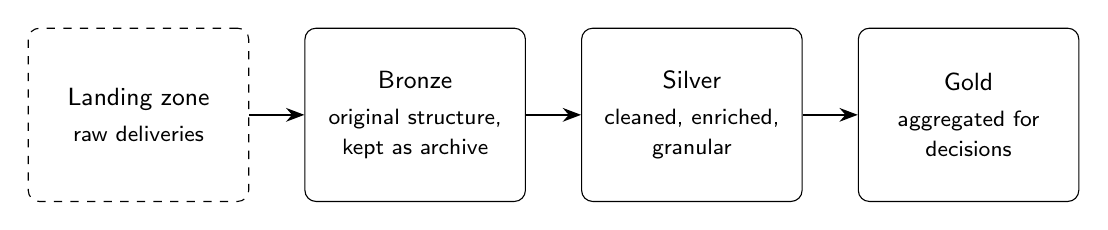
\begin{tikzpicture}[
		layer/.style={draw, rounded corners, align=center, minimum width=2.8cm, minimum height=2.2cm, font=\small},
		flow/.style={-{Stealth}, thick}]
		\node[layer, dashed] (land) {Landing zone\\[2pt]\footnotesize raw deliveries};
		\node[layer, right=0.7cm of land] (bronze) {Bronze\\[2pt]\footnotesize original structure,\\\footnotesize kept as archive};
		\node[layer, right=0.7cm of bronze] (silver) {Silver\\[2pt]\footnotesize cleaned, enriched,\\\footnotesize granular};
		\node[layer, right=0.7cm of silver] (gold) {Gold\\[2pt]\footnotesize aggregated for\\\footnotesize decisions};
		\draw[flow] (land) -- (bronze);
		\draw[flow] (bronze) -- (silver);
		\draw[flow] (silver) -- (gold);
	\end{tikzpicture}
	\caption{The Medallion architecture with its three layers -- Bronze, Silver and Gold -- and the landing zone in front of them, after \textcite{Strengholt.2025}.}
	\label{fig:medallion-architecture}
\end{figure}

\subsubsection{Landing zone}

% Landing zone
A landing zone\footnote{Alternative names are ``tin layer," ``pre-Bronze," ``pre-refinement," ``staging area," or  ``landing area".} is used as a preliminary area, where raw data is ingested before it lands in the Medallion architecture. This is useful when dealing with external services, where it is necessary to have a secure area to temporarily store data before processing it further. In the area of financial supervision this includes, among others, data submitted by supervised entities or data received via ESMA's TRACE API. While the Bronze layer mainly serves as the area for data collection, using a landing zone can be useful in larger or more complex environments. Thus, where and how to use it depends on an organization's requirements \parencite{Strengholt.2025}. For example, where data comes from multiple sources, in batches and in a less optimal file format -- like in the case of EMIR and similar reporting data sets -- a landing zone is a good approach to organize data ingestions. By contrast, exchange rate data from European Central Banks is rather small and can be directly imported into the Bronze layer.


\subsubsection{Bronze layer}

% Bronze layer
The Bronze layer acts as the zone for raw data collected from various sources. Data in this layer is stored in its original structure without any transformation, serving as a historical record and a single source of truth. It ensures data is reliably captured and stored, making it available for further processing, but also as a queryable archive for raw data \parencite{Strengholt.2025}. For larger data sets such as EMIR and SFTR this implies that data is not stored as XML files in the Bronze layer, but rather converted into a performant file format like Parquet or Delta Lake without changes to the original schema, although minor changes with respect to the header files might be warranted in combination with a metadata store.

The transition from the landing zone to the Bronze layer usually includes steps like decompressing zipped files, comparing checksums, generating metadata, and file conversion into a more performant file format. Furthermore, this step can include the classification or encryption to protect sensitive information, which is the case for personal information reported under MiFIR.

With respect to the organisation of files within the Bronze layer, \emph{fincommons} follows an established practice to organize files by the source of the data and its content \parencite{Gorelik.2019}. More detailed information on how this is implemented for an individual data set can be found in the following chapters.

\subsubsection{Silver layer}

% Silver layer
The Silver layer ``refines and standardizes raw data for complex analytics through quality checks, standardization, deduplication, and other transformations. It acts as a transitional stage for processed, granular data with improved quality and consistency." \parencite[p.~5]{Strengholt.2025} Designing the Silver layer ``is often a hot topic, as there are many possibilities. It is significantly influenced by the number of data sources collected, the extend to which these sources share the same key elements or objects that can be matched, related, and combined across different source systems, and the need to harmonize the overlapping key elements for an integrated perspective." \parencite[p.~66]{Strengholt.2025}

Within \emph{fincommons} the design of the Silver layer is mainly determined by the requirements of the main consumers of the data in this layer. This group comprises experts, who are sufficiently qualified to independently work with the data. This entails mainly sufficient domain knowledge, but might also include the necessary technical expertise to efficiently work with large datasets, where this is advisable. And since the focus of this group is assumed to be on answering business and supervisory questions -- regularly under considerable time pressure -- rather than implementing data pipelines, data in the Silver layer should be prepared accordingly. However, it is important to highlight that this does not include major transformations or aggregations, but rather denormalization, enrichment and enforcement of naming and format conventions. In short, the overarching goal of the Silver layer within \emph{fincommons} is to provide technically skilled domain experts with highly granular data in an intuitive structure, which serves as the departure point for data science and analytics projects.

Similar to the Bronze layer, data in the Silver layer is organised within a traditional data lake architecture. How a table of either layer is laid out on disk -- whether it is cut into partitions, and how large its files are -- is a separate question from the logical design of the layer, and one with a considerable effect on the cost of running a pipeline. It is discussed in section \ref{sec:intro-data-layout}.

\subsubsection{Gold layer}

% Gold layer
Finally, the ``Gold layer optimizes refined data for specific business insights and decisions. It aggregates, summarizes, and enriches data for high-level reporting and analytics, emphasizing performance and scalability to provide fast access to key metrics and insights."\parencite[p.~5]{Strengholt.2025} Whereas data in the Bronze or Silver layer might be used on a relatively irregular basis, data in the Gold layer is supposed to be used regularly via highly standardised channels by domain experts without advanced data processing knowledge. From a data processing perspective, this entails a strong focus on performance, efficiency and accessibility, which is a core strength of traditional data warehousing. Therefore, larger data sets in the Gold layer are usually normalised and follow a star schema, which should ensure compatibility with popular data visualisation tools.

Within \emph{fincommons}, tables in the Gold layer are created based on business requirements, which in the field of financial data work can be grouped into two general domains: data quality assurance and risk analysis.\footnote{For a more detailed taxonomy of supervisory domains see, for example, \url{https://digitaltransformationsolutions.io/wp-content/uploads/2025/09/DTS-SupTech-Taxonomy.pdf}.} For the purpose of data quality assurance, Gold layers generally include various tables containing information on the quality of reports. The purpose of those tables is to assist supervisors in identifying entities where supervisory action might be warranted to improve overall data quality -- or to assist a firm in finding the problems in its own reports before it submits them. This is achieved by running various data quality checks on the data in the Silver layer. The results of those checks are stored in a table \emph{issues}. This table can be combined with information from the Silver layer and the entity master data described in chapter \ref{ch:entitymasterdata} to produce tables that can be used for data quality monitoring. This can entail specific tables for entity-level and overall data quality developments. Moreover, tables are structured in a way that allows for use in dashboards without computationally overwhelming the user interface. Thus, they contain aggregated information.\footnote{For example, table \emph{general} may only include the top N entities with the most data quality issues and all other entities are summarised in the category ``Other". The same can be done with the identified issues. This ensures that the cardinality of a column remains limited and, hence, improves performance.} Finally, the data quality section of a Gold layer can contain data that could be sent back to reporting entities in order to help them to understand the identified problem, identify its source and correct it.

With respect to risk analysis, tables are tailored based on business requirements. In the field of financial data work, this usually includes views for individual entities and general market developments. Analogously to data quality assurance, the overarching goal of those views is to assist their users in detecting potential issues that might warrant further attention. On the one hand, this can include backward-looking monitoring of compliance-relevant information. On the other hand, this might include the results of forward-looking stress tests. However, since the creation of Gold layer tables strongly depends on individual use cases, more detailed treatments of the topic are postponed to the respective data-specific chapter below.\footnote{\textcite[Chapter 7]{Strengholt.2025} covers the design of the Gold layer. Inspiration for how to approach the design of a dashboard can be found in \textcite{Wexler.2017}, but it does not cover data-related issues.}

\subsubsection{Work Layer}

Data lake architectures sometimes also mention a ``work" or ``analytics" layer, which describes the place where data scientists or data engineers can temporarily store data to develop new solutions or perform one-off analysis. ``This zone can be organized by user, by project, by subject, or in a variety of other ways." \parencite{Gorelik.2019}

Since this layer is used for development and data experimentation, it is not further considered in this handbook.

\subsection{Potential interactions with existing data infrastructures}

% Overview
Figure \ref{fig:framework-overview} summarises the design pattern of the framework and its potential interaction with already existing data infrastructures. The right side of the figure represents a highly stylised data process that is already implemented within an organisation. It starts by importing data from various sources and processing it within a certain data infrastructure. The data is subsequently used for internal data products like dashboards and reports, which serve its analytics. Note that the grouping ``existing infrastructure" also indicates that every group element -- i.e., data pipelines, dashboards and (automated) reports -- is developed and hosted exclusively within an individual organisation. In general, \emph{fincommons}, which is shown in the bottom left of the diagram, follows the same logic of ingesting, processing and analysing data. Moreover, the grouping \emph{fincommons} also indicates that data models and code are developed jointly within the framework. There are only two relevant differences compared to the grouping ``existing infrastructure": First, from a software design and data model perspective, \emph{fincommons} is specifically designed with the goal of facilitating code-sharing. Second, there currently is no ``Dashboard" component within that grouping, since this would entail making many further strategic decisions regarding specific dashboarding technologies. While nothing prevents willing organisations to add this functionality to the \emph{fincommons} codebase in the future, for now the framework's focus is on data preparation pipelines and (semi-)automatised reports.

The interaction of the \emph{fincommons} with existing data infrastructures can be handled very flexibly. In a scenario, where only the analytical functionality of the framework should be used, local data engineers would have to load relevant data into the Silver or Gold layer as specified in the documentation of an analytics use case. After that, functions of the accompanying Python or R package can be executed to perform further data processing into the Gold layer and generate standardized reports. Similarly, if an organisation wishes to gradually increase the usage of the framework for its data processing jobs, this can be done by loading data into the respective folders as specified in the documentation and executing the Python package's data processing functions.


\begin{figure}[h]
	\centering
	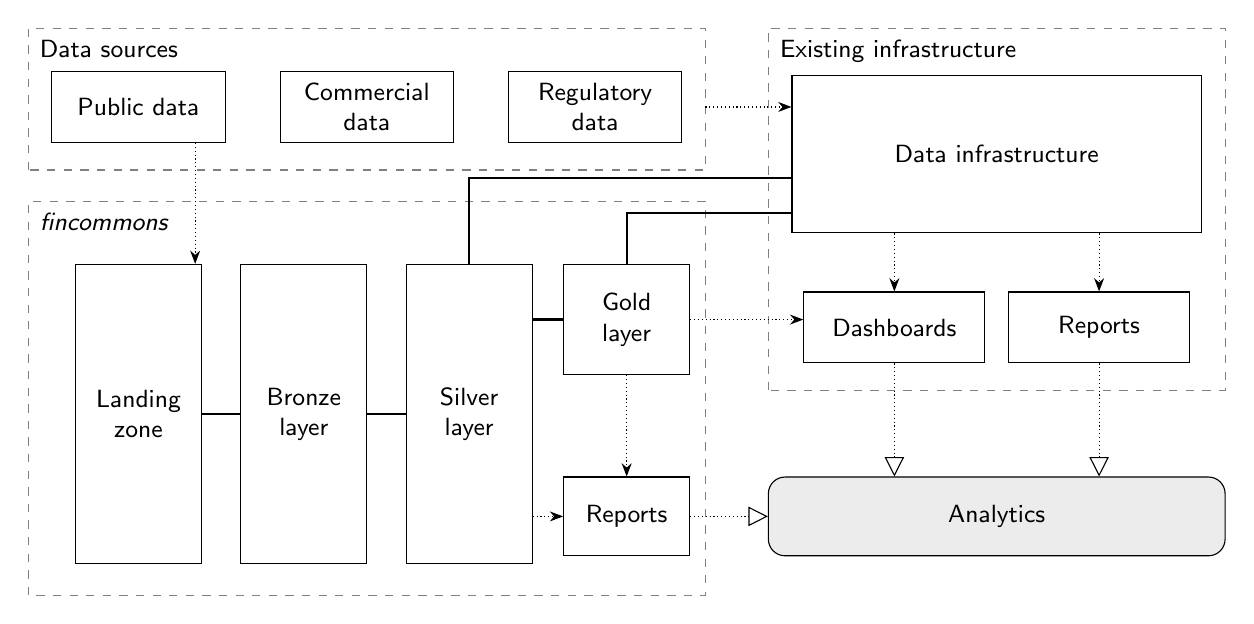
\begin{tikzpicture}[
		x=1cm, y=1cm, font=\small,
		group/.style={draw, dashed, gray},
		grouplabel/.style={anchor=north west, inner sep=4pt},
		box/.style={draw, align=center, inner sep=2pt},
		flow/.style={-{Stealth}, densely dotted},
		serves/.style={-{Triangle[open, length=7pt, width=7pt]}, densely dotted},
		link/.style={thick}]
		% Groups
		\draw[group] (0, 5.4) rectangle (8.6, 7.2);
		\node[grouplabel] at (0, 7.2) {Data sources};
		\draw[group] (9.4, 2.6) rectangle (15.2, 7.2);
		\node[grouplabel] at (9.4, 7.2) {Existing infrastructure};
		\draw[group] (0, 0) rectangle (8.6, 5.0);
		\node[grouplabel] at (0, 5.0) {\emph{fincommons}};
		% Data sources
		\node[box, minimum width=2.2cm, minimum height=0.9cm] (public) at (1.4, 6.2) {Public data};
		\node[box, minimum width=2.2cm, minimum height=0.9cm] (commercial) at (4.3, 6.2) {Commercial\\data};
		\node[box, minimum width=2.2cm, minimum height=0.9cm] (regulatory) at (7.2, 6.2) {Regulatory\\data};
		% Existing infrastructure
		\node[box, minimum width=5.2cm, minimum height=2.0cm] (infra) at (12.3, 5.6) {Data infrastructure};
		\node[box, minimum width=2.3cm, minimum height=0.9cm] (dashboards) at (11.0, 3.4) {Dashboards};
		\node[box, minimum width=2.3cm, minimum height=0.9cm] (reports-ext) at (13.6, 3.4) {Reports};
		% fincommons
		\node[box, minimum width=1.6cm, minimum height=3.8cm] (landing) at (1.4, 2.3) {Landing\\zone};
		\node[box, minimum width=1.6cm, minimum height=3.8cm] (bronze) at (3.5, 2.3) {Bronze\\layer};
		\node[box, minimum width=1.6cm, minimum height=3.8cm] (silver) at (5.6, 2.3) {Silver\\layer};
		\node[box, minimum width=1.6cm, minimum height=1.4cm] (gold) at (7.6, 3.5) {Gold\\layer};
		\node[box, minimum width=1.6cm, minimum height=1.0cm] (reports-fc) at (7.6, 1.0) {Reports};
		% Analytics
		\node[box, rounded corners=6pt, fill=gray!15, minimum width=5.8cm, minimum height=1.0cm] (analytics) at (12.3, 1.0) {Analytics};
		% Data flows
		\draw[flow] ([xshift=0.72cm]public.south) -- ([xshift=0.72cm]landing.north);
		\draw[flow] (8.6, 6.2) -- (infra.west |- 0, 6.2);
		\draw[link] (landing) -- (bronze);
		\draw[link] (bronze) -- (silver);
		\draw[link] (silver.east |- gold.west) -- (gold.west);
		\draw[link] (silver.north) |- (infra.west |- 0, 5.3);
		\draw[link] (gold.north) |- (infra.west |- 0, 4.85);
		\draw[flow] (gold.east) -- (dashboards.west |- gold.east);
		\draw[flow] (gold.south) -- (reports-fc.north);
		\draw[flow] (silver.east |- reports-fc.west) -- (reports-fc.west);
		\draw[flow] (infra.south -| dashboards.north) -- (dashboards.north);
		\draw[flow] (infra.south -| reports-ext.north) -- (reports-ext.north);
		% What serves the analytics
		\draw[serves] (dashboards.south) -- (dashboards.south |- analytics.north);
		\draw[serves] (reports-ext.south) -- (reports-ext.south |- analytics.north);
		\draw[serves] (reports-fc.east) -- (analytics.west);
	\end{tikzpicture}
	\caption{Design pattern of the framework and its potential interaction with existing analytics infrastructures. \emph{fincommons} implements the part labelled \emph{fincommons} for public data; packages of pipelines on supervisory reporting data implement it for those data.}
	\label{fig:framework-overview}
\end{figure}


\section{Technological considerations}


\subsection{Programming languages}

% Languages
In principle, library-based code-sharing can be done in any programming language. However, as data processing and cleaning constitute the main part of analytical data work, it is prudent to focus on those languages, which are predominantly used for those purposes. Currently, Python and R are powerful open-source programming languages, which enjoy great popularity among practitioners. The \emph{fincommons} codebase reflects this in two ways: First, given Python's enormous popularity in the fields of data engineering, machine learning and artificial intelligence as well as its increasing adoption by European and national supervisory authorities and by financial firms, functions for the transition of data between different layers are implemented in Python. Second, given R's strengths for statistical modelling and data visualisation, R-scripts and R-markdown reports can be used for the fast development and sharing of ad-hoc analyses.

\subsection{Spark and open table formats\label{sec:intro-data-formats}}

Apache Spark serves as the backbone of data pipelines which handle large data sets.\footnote{See \url{https://spark.apache.org/}.} It is versatile, highly popular in the international data community, and works both on laptops as well as clusters. This makes it attractive for use within \emph{fincommons}, where out-of-the-box usability implies that its users should be able to run code quickly, irrespective of their current hardware stack.

Spark alone, however, does not settle how the data of the Medallion architecture is stored. Parquet is an efficient columnar file format, but a directory of Parquet files is not a table. It has no notion of a transaction, so a reader that arrives while a data set is being rewritten sees whichever files happen to exist at that moment, and it has no notion of a row that is updated, so a correction can only be expressed by rewriting the partition it falls into. Both limitations are binding in regulatory data work. The tables that a nightly pipeline rebuilds are the same tables a monitoring dashboard reads, and reporting data is revised as a matter of course: resubmissions, cancellations and late deliveries are the normal case rather than the exception.

This gap is closed by open table formats, which maintain a transaction log beside the Parquet files and thereby turn a directory into a table with atomic commits, snapshot isolation and row-level updates. The two established open-source candidates are Delta Lake, hosted by the Linux Foundation, and Apache Iceberg.\footnote{See \url{https://delta.io/} and \url{https://iceberg.apache.org/}.} Both store their data as Parquet, both are supported by Spark, and both meet the requirements stated above, so the choice between them does not follow from those requirements alone.

The current implementation of \emph{fincommons} uses Delta Lake, for three reasons that concern the situation of the institutions using it rather than the merits of the two formats.

First, a table has to be addressable by path as well as through a catalogue. The framework is meant to run unchanged on an analyst's workstation and on a cluster, and a path is the one address that means the same thing in both places: a directory of the local file system in the first case, a location in a volume or in object storage in the second. Where a catalogue exists, a layer of Delta tables can instead be addressed by catalogue name, the address Unity Catalog governs; which of the two a layer uses is decided by the configuration file alone. Delta treats a path-addressed table as the ordinary case and a catalogued one as an option. Iceberg is designed around a catalogue that mediates between the name of a table and its current metadata, which is an advantage for an organisation running several query engines against one metastore, but an additional component to operate for an institution that wants to run a pipeline on a laptop first and decide about a data platform afterwards.

Second, the reference deployment of the framework is a Databricks environment, where Delta is part of the runtime and needs no configuration at all, while off-cluster it is one additional package. Choosing the format that the target platform treats as native removes a class of configuration problems from the code that the recipients of the framework have to run.

Third, the format has to be readable without Spark. An analyst who wants to inspect a table in an ad-hoc script should not have to start a Spark session in order to do so, and part of the analytical work of the framework is done in R rather than in Python. Implementations of the Delta protocol outside the JVM are available for that purpose: the \verb|deltalake| package reads such tables directly, as does Polars through it, on which the Python package already depends.

None of this is an argument that an institution which has already standardised on Iceberg should change course, and the decision is a shallower one than it appears. The format is named in two shared modules, \emph{addressing} and \emph{storage}, which open and write the tables of the Silver layer for every module. Only the FIRDS module refers to it more widely, because its historical database is updated with MERGE statements instead of being rewritten. Porting the framework to another table format is therefore a bounded exercise. The two formats have moreover been converging, in that the metadata of a table written in one of them can increasingly be exposed in the dialect of the other, so that the storage decision constrains the choice of query engine considerably less than it did when the formats first appeared.


\subsection{Physical layout of a table\label{sec:intro-data-layout}}

Choosing an open table format settles how a table is addressed and updated, but not how its rows are distributed over the files that hold them. That question is easy to answer badly, because the intuition that suggests the wrong answer is a reasonable one, and because the cost of the wrong answer does not appear in a small test run. Since the pipelines of the package are meant to be run by institutions on data of very different sizes, the following considerations are worth stating once in general terms.

The first concerns \emph{partitioning}, i.e. cutting a table into one directory per value of a chosen column. Partitioning is attractive because it appears to offer parallelism and pruning at no cost, and a categorical column such as a country, a trading venue or a counterparty type suggests itself. Neither benefit is automatic. Pruning only materialises where the queries and updates that actually run restrict the partition column to a few of its values; where a daily update touches most of them at once, as a delta file of a reporting regime typically does, every partition is read regardless and the partitioning has bought nothing. Parallelism, in turn, comes from the number of files and the size of the data, not from the number of directories. What partitioning does cost is a fixed overhead per partition and, more importantly, a multiplication of the number of files written: an append writes at least one file per combination of writing task and partition value, so a table with a few hundred partition values written by a few hundred tasks receives tens of thousands of files from a single update. A workable rule of thumb is not to partition a table below roughly a terabyte, and to check the average size of a partition before choosing a column: partitions well below a gigabyte are a sign that the column is too fine.

The second concerns \emph{file size}, which is the quantity that actually governs the cost of reading a table. Every file must be opened, its footer parsed and its statistics evaluated, and this cost is paid per file rather than per row. A table of a given size therefore becomes progressively more expensive to read as the same data is spread over more files, and a pipeline that appends to a table daily accumulates files at a constant rate while the cost of each update grows with the number accumulated so far. A backfill over several years of history then degrades quadratically, which is the characteristic signature of the problem: the pipeline is not uniformly slow but becomes slower the longer it runs. The remedies are to let the table format size the files of a write, which Delta does when the \verb|optimizeWrite| property is set, and to run the format's compaction routine periodically.

Most tables of the framework are not Delta tables but plain Parquet, partitioned by a reference date and appended to one date at a time, and for them neither remedy is available, since both live in the transaction log. The problem is nevertheless the same. The frame that reaches the write has typically been through joins and window functions, each of which spreads its rows over the tasks of a shuffle, so that a single reference date of a reporting regime's contract table can arrive as up to two hundred files of a fraction of a megabyte each, all of which every query over a period has to open. The framework therefore applies Spark's \verb|rebalance| hint to every partitioned Parquet write, through the function \verb|rebalanced| of the module \emph{layout}. The hint adds one shuffle by the partition columns, after which adaptive query execution merges the small partitions of that shuffle and splits the large ones to an advisory size, so that a small date is written as one file and a large one as a few of a sensible size. The two obvious alternatives are worse: \verb|coalesce| saves the shuffle but runs every step before it, window functions included, in as few tasks as it leaves, and a fixed \verb|repartition| is wrong for every date that is unusually large or small. A table that holds small files nonetheless, whatever left them behind, is rewritten by \verb|compact_partitions| of the same module. It rewrites each partition into a folder beside it, compares the number of rows, and only then swaps the two folders. Without a transaction log that swap consists of two renames rather than one commit, so the function is meant to run while nothing writes the table and nothing important reads it, and a run that dies between the renames is completed by the next one.

The third concerns what replaces partitioning where data skipping is genuinely wanted. Modern table formats offer \emph{clustering}, which orders the rows within files by one or more columns and records the range each file covers, so that the statistics of a file can exclude it from a scan. This achieves what partitioning was supposed to achieve, without cutting the table into directories and therefore without the file multiplication, and it permits several columns where partitioning realistically permits one. The natural clustering key is the set of columns that the updates of the table match on. Where a table is maintained with MERGE statements, as the FIRDS historical database is, keeping the clustering key and the merge condition in step is worth enforcing in the code itself, since the two can otherwise drift apart silently as a pipeline is maintained.

A fourth point concerns the quantity that the first two refer to as the number of writing tasks, since it is the one of the four that is set rather than inherited. A write produces at least one file per task that participates in it, and the number of tasks after a shuffle is fixed by the configuration setting \verb|spark.sql.shuffle.partitions|, whose default of 200 is chosen for a cluster. On a workstation this cuts every shuffle into far more tasks than there are cores to run them on, and the scheduling of a task costs the same whether it carries a million records or none. It is also the factor that the file multiplication of a partitioned table is proportional to: two hundred tasks writing into a few hundred partition directories is precisely how a single update comes to leave tens of thousands of files behind. Adaptive query execution, which is enabled by default in current versions of Spark, coalesces partitions after a shuffle and thereby removes part of the problem, but it does not reduce the number of tasks a shuffle is planned with, so the setting is still worth choosing deliberately. It should be derived from the cores the session actually has rather than fixed to a number, so that the same code behaves reasonably on a laptop and on a cluster; twice the available parallelism is a serviceable starting point. Unlike the memory of the driver, this setting can be changed after the session has started, which is what makes deriving it possible at all.

A general observation applies to all four points. The cost of a poor physical layout is invisible in the small test runs by which a pipeline is usually developed, and becomes dominant only at the volumes at which it is eventually operated. Where a pipeline is unexpectedly slow, the number of files a table consists of, their average size and the number of tasks its writes are cut into are therefore among the first quantities to inspect, and they are cheap to obtain. The FIRDS chapter reports a case in which this diagnosis applied, together with the measurements that settled it.


\subsection{Reading semi-structured data under a declared schema\label{sec:intro-data-schema}}

Regulatory data arrives as XML far more often than as anything else, and a pipeline that reads it has a choice between letting the reader infer a schema from the file and declaring one in advance. Declaring one is the better practice and the framework does so throughout: an inferred schema varies with the contents of the particular file, so a field absent from one day's delivery silently changes the shape of the table built from it, and inference costs a full pass over the data before any of it is read. A declared schema fixes the shape once, and naming only the paths a pipeline actually uses makes it indifferent to the greater part of a specification it never touches.

The property that makes a declared schema safe is also the one that makes it quiet, and it is worth stating plainly: a reader given a schema discards what the schema does not name, and reports an element it was not asked for in exactly the same way as an element the file did not contain, namely as an empty value. Nothing distinguishes the two downstream. Where the unnamed element is one the pipeline has no use for, that is precisely the desired behaviour. Where it is one the pipeline depends on, the pipeline is not reading the data it believes it is reading, and it will not be told.

The situation in which this arises is not exotic. ISO 20022, which most European reporting formats are expressed in, makes heavy use of the \emph{choice}: a period may be stated as a start date, or as an end date, or as a range holding both, and a reporting party may exercise the choice differently for different kinds of record within one file. A pipeline that names one branch and not the others reads a well-formed file and obtains nothing from a third of it. The remedy is not to abandon the declared schema but to name every branch a choice admits and to reconcile them where the value is used, which costs one expression per field and removes the failure mode entirely. Section \ref{sec:firds-bronze} describes a case of this kind.

What turns such an omission from a defect into an expensive one is the second property: an empty value does not stop anything. It flows into whatever is computed from it, and the arithmetic of dates in particular propagates it without complaint -- the day before an unknown day is unknown. A record carrying it is written, a table accepts it, and an invariant the pipeline depends upon is quietly broken. The eventual failure occurs at the first operation that cannot tolerate the broken invariant, which may be several runs later and in a component with no connection to the one at fault, and the error it raises describes the symptom. Diagnosing it costs far more than the original omission suggests.

The conclusion generalises beyond XML and beyond any particular format. Where a value is not merely carried but relied upon -- because a key, a validity period or an ordering is derived from it -- its absence should be refused at the point where the record enters the pipeline, with a message naming the records concerned. A check of this kind is cheap, it runs where the cause still is, and it converts a class of silent corruption into a run that stops and says why. It is the same argument that applies to a data set received from a third party, and it is made in that context in section \ref{sec:intro-logging}: a pipeline whose failures are loud is worth more than one whose failures are rare.


\subsection{Naming conventions\label{sec:intro-data-naming}}

A name given to a file, a directory or a column rarely stays where it was given. The directory a table is written into becomes the name the table is registered under, the name of a column of the Silver layer is the name an analyst types into a query, and a file shipped with the package is addressed by a string in the code that loads it. Because a name travels in this way, what it may contain is not decided by the place it is first written down but by the most restrictive place it can eventually arrive at, and that place is the catalogue rather than the file system.

File systems accept almost anything, and a hyphen in a file name is unobjectionable there. SQL identifiers are considerably stricter. In Databricks Unity Catalog, as in most SQL dialects, an identifier containing a hyphen has to be enclosed in backticks wherever it appears, because the hyphen would otherwise be read as an operator; in some positions such a name is not permitted at all. The convention the platform's own objects follow is \emph{snake\_case}, that is, words separated by underscores. A name written with underscores therefore passes unchanged from a file, through a directory, into a table, a view or a column, whereas a name written with hyphens has to be quoted or rewritten at the first boundary it crosses, and every consumer of it has to remember to do so.

The \emph{fincommons} framework accordingly uses underscores rather than hyphens throughout, including in the files it ships in its own data directory, such as the reconstructed schemas that the Bronze layer readers are given. This is a convention rather than a technical necessity, and for a file that is only ever opened by name it makes no difference whatsoever. Its value lies in removing the question: a contributor who never has to decide whether a particular name will cross into a catalogue cannot decide it wrongly.

The cost of the opposite choice is modest but it is paid late. A hyphenated name is harmless until the day it is used as an identifier, at which point it is corrected not in one place but in every place that refers to it -- the code that loads the file, the tests that assert on it, and the documentation that reproduces the command it was generated with. Renaming is mechanical and safe as long as the references are literal strings, which is a further reason to address a shipped file by a plain constant rather than to assemble its name at run time from parts.


\subsection{Quarto for replicable analyses}

While dashboards are suitable choices for visualising highly standardised information, adapting them to new requirements can take time and might involve changes to the data pipeline. By contrast, analytics notebooks can be adapted quickly and allow for more complex and differentiated visualisations and analyses. Currently, a popular notebook format are Jupyter\footnote{See \url{https://jupyter.org/}.} or Quarto\footnote{See \url{https://quarto.org/}.} notebooks. Jupyter notebooks are very popular in the Python community. However, there seems to be no way to hide the code of an analysis, which is desirable in case results should be communicated to the management quickly. By contract, Quarto documents allow to hide code. They also can be used to create different output formats such as static PDF or interactive HTML reports and they can handle different programming languages. Hence, within the \emph{fincommons} code base, Quarto notebooks are currently the preferred solution for sharing analytical work.


\section{Software architecture\label{sec:intro-software}}

% Libraries & documentation



% Professional code development
Overall, the software architecture of \emph{fincommons} is modular and closely aligned with the underlying data architecture and associated analytical use cases. In this regard, the accompanying code should follow established best practices in code development such as ``separation of concerns" and ``don't-repeat-yourself", regardless of the chosen programming language. This should make the resulting systems operable, simple and evolvable \parencite[Chapter~1]{Kleppmann.2017}.


\subsection{Code security}

A major concern in software development is code security. Since \emph{fincommons} packages in Python and R heavily rely on a number of other third-party software libraries, it is prudent to check whether external code meets an institution's internal IT security requirements. There exists a range of proprietary and open-source software composition analysis (SCA) solutions, which can be integrated with internal code repository tools and perform those checks automatically.\footnote{See, for example, \url{https://en.wikipedia.org/wiki/Software_composition_analysis} for further references.}. Against the background of a multitude of available SCA solutions, their ability to work directly on the source code and the technology-agnostic approach of \emph{fincommons}, this topic is currently considered to go beyond the scope of this handbook. However, future versions could elaborate more on solution-independent aspects, which are beyond the knowledge of the current author.

Note that since all of the packages used in the accompanying code are widely used across the globe, there seems to be no strong indication that would warrant serious security concerns. Nevertheless, such an assessment has not been performed by the current author of the accompanying packages.

%\begin{figure}[h]
%	\centering
%	\includegraphics[height=8cm]{archimate-data-processing-general}
%	\caption{Default pattern of the transition between the landing zone and Bronze layer using the ArchiMate modelling language.}
%	\label{fig:archimate-data-processing-general}
%\end{figure}


\section{Logging\label{sec:intro-logging}}

A data pipeline runs unattended. It is started by a scheduler at night, it processes deliveries that an institution has no control over, and by the time anyone looks at the tables it produced, the process that produced them no longer exists. Whatever the run recorded about itself while it was running is therefore the only account of it that remains, and the question an analyst eventually has to answer about a figure in a report -- which delivery it came from, whether every file that should have been processed was processed, and whether anything was quietly set aside -- can only be answered from that account.

The point deserves emphasis because the obvious alternative is so convenient. A pipeline under development is run interactively, its progress is printed to the console, and the printed lines are read by the person who started it. Nothing about that arrangement announces its own failure when the same code is later scheduled: the lines are still produced, they are still collected by the platform, and they are still, in a narrow sense, available. What is lost is everything that makes them usable at a distance. A printed line carries no time stamp, so the order of two events can be inferred but their spacing cannot; it carries no severity, so a note that a table was rebuilt is indistinguishable from a report that a file could not be read; and it carries no indication of which pipeline, which layer or which reference date it concerns, so a log covering a night of several pipelines cannot be separated back into them. The remedy is not to print more, but to record instead of printing.

\subsection{Levels}

The framework uses the levels of the Python standard library, and fixes what each of them asserts about a run, so that a reader can decide what to do from the level alone without reading the message.

\textsc{Info} is the record of what the run did: which stage started and finished, how long it took, which reference dates were applied, how many findings were written. This is the level a scheduled job runs at, and the material from which the history of a table can be reconstructed afterwards.

\textsc{Warning} states that the run remained valid but did less than a reader might assume. An update that found no new delta file to apply, a source whose data ends earlier than the others and thereby holds back the combined table, a file whose schema the import does not recognise: in each case the pipeline finished successfully, and in each case the tables afterwards look exactly as they would look had there been nothing to do. The distinction exists only in the log, which is precisely why it has to be there.

\textsc{Error} is reserved for a unit of work that failed while the run carried on by design. The import of reference data files is the case that motivates the level: files arrive in bulk from a third party, and a single malformed file must not abandon the files behind it in the folder, so the offending file is moved aside and the loop proceeds. The decision to continue is deliberate, but it is only defensible if what was set aside is recorded, with the underlying exception and its traceback, and if the number of such files is reported at the end of the run. An import that quarantines every file it was given otherwise finishes successfully and looks, from the state of the data lake, exactly like an import that had nothing to do.

\textsc{Debug} carries the detail needed to reproduce a run rather than to monitor it, and is switched off by default.

\textsc{Critical} is not used at all, and its absence is the substantive point of the scheme. A problem that invalidates the result of a run must interrupt that run, not describe it. The framework accordingly raises an exception wherever a pipeline can no longer do its work correctly -- when the historical database carries no watermark, so that there is no way to tell which deliveries have already been applied, or when a table cannot be read at all, which must never be mistaken for a table that is empty. Logging is never the mechanism by which a pipeline decides that it may continue. Where a stage does fail, the failure is recorded with its traceback and the exception is re-raised unchanged, so that the scheduler sees the run as failed and the log explains why.

\subsection{Context}

Anything by which a record may later have to be filtered or grouped is recorded beside the message rather than inside it. Each record of a pipeline therefore carries the module it came from, the layer it was working on, and, where they apply, the source, the table, the reference date, the file and the number of rows. A line of the log reads as a constant sentence followed by the circumstances of that particular occurrence:

\begin{quote}
\small
\verb|2026-09-08 03:14:22 INFO  fincommons.firds.silver  Applied delta file|\\
\verb|    module=firds layer=silver table=MAIN datadt=2026-09-04 rows=18432|
\end{quote}

The arrangement costs nothing at the point of writing and buys two things. Because the sentence does not vary with the run, every occurrence of the same event can be collected by matching one constant string, which is not possible when the reference date has been formatted into the middle of it. And because the circumstances are held as separate fields rather than as prose, the same records can later be emitted as structured data for a log platform without a single line of the pipelines being touched.

\subsection{Operating the log}

Two conventions keep the arrangement workable in the environments the framework is meant to run in.

The first is that the library configures nothing. Modules obtain a logger and write to it; no module attaches a destination, sets a level or configures anything on import. That decision belongs to whoever runs the code, because a package that configures logging on import overrides the arrangements of the notebook or the scheduled job that imported it, and does so invisibly. A single function is provided for the purpose and is called by the entry points. On a managed platform such as Databricks, where the driver already collects the standard error of the process, it is enough to raise the level of the framework's own logger and let the platform do the collecting.

The second is that logging does not displace the ordinary output of a program. The demonstration scripts that accompany the analytical modules print result tables for a person watching the console; those tables are the output of the program and remain on standard output, while the log goes to standard error. The distinction is easy to apply in practice: a statement that would still be useful in a log file three weeks after the run belongs in the log, and a statement that only makes sense to someone watching the terminal at that moment does not.

Finally, because the level of a record is a claim about the run rather than a matter of presentation, the framework tests it. The behaviours that exist only in the log -- an update that found nothing to apply, a delivery that was quarantined -- are asserted in the test suite like any other behaviour, which is what keeps them from being quietly lost the next time the surrounding code is rewritten.

\section{Continuous integration and delivery}

Development practices only take effect if they are applied to every change, rather than to those a contributor remembers to check. This is the purpose of continuous integration: every change proposed to the shared codebase is built, and its tests are executed, automatically and on a neutral machine before the change is merged, so that the state of the shared code is known at all times instead of being assumed.

For a code-sharing framework the argument for this practice is stronger than the general one. Section \ref{sec:intro-motivation} argued that code-sharing among institutions rests on trust, and that a lack of trust creates strong incentives for continued local development. An institution that installs a package contributed by another institution cannot realistically audit it, and it should not have to. What it can do is see whether the package is covered by tests and whether those tests are executed on every change. Continuous integration is thus the mechanism that turns a claim about the quality of shared code into something a recipient can verify without reading the code itself. The Python package accompanying this handbook currently carries several hundred automated tests across its modules, which are the natural content of such a pipeline.

A constraint of the regulatory context is that no confidential data -- neither reporting data nor a firm's own books -- may enter such a pipeline. Tests therefore have to run against data that could be published: fixtures written into the test itself, or synthetic data generated by the package. The \emph{fincommons} codebase follows this rule. The tests of the exchange rate module never contact the websites of the ECB or the BIS, but exercise the module against an archive of their own. Besides making automated testing possible at all, this has the useful side effect that any recipient of the code can reproduce the entire test suite, which would not be the case for tests that depend on data an institution is not permitted to share.

The delivery half of the practice is the automated production of a versioned, installable artefact from a given state of the source code, so that the artefact which was tested and the artefact which is installed in an analytical environment are demonstrably the same one. Note that the term is deliberately continuous \emph{delivery} and not continuous \emph{deployment}. Promoting a new version automatically into an environment that processes confidential data is rarely acceptable, and the release into production should remain a decision that a person takes and records. What automation can remove is the manual work of building, testing and packaging that precedes that decision, not the decision itself.

\section{Infrastructure as code}

A data pipeline does not run in a vacuum. It requires storage with a particular directory or volume layout, a compute environment with a particular runtime version, the libraries it depends on, and permissions that allow it to read and write what it should and nothing else. Traditionally this environment is created by hand, through the web console of a cloud provider or through a ticket to an infrastructure team, and it exists thereafter only as settings that no one can inspect as a whole. Infrastructure as code is the practice of describing that environment in declarative files, which are kept in a version control system next to the source code, and of leaving it to a tool to reconcile the actual environment with the description.\footnote{A widely used tool of this kind is Terraform, see \url{https://www.terraform.io/}. Most platform vendors additionally provide equivalents specific to their own products.}

For \emph{fincommons} this is more than a general recommendation, because the promise of the package is that an analysis performed by one institution can be reproduced by another. That promise covers the code and the data model, but the result of a computation also depends on the environment in which it ran, i.e. on the runtime version, the versions of the libraries and the layout of the data lake. Where the environment is described in files, that description can be shared alongside the code, and a receiving institution can recreate an equivalent environment instead of reconstructing it from a prose account of which buttons to press.

The design of the accompanying Python package reflects the resulting division of responsibilities. Each module provides a function that creates the directory tree of its part of the data lake, which is convenient on a workstation, but those functions are explicitly documented as being meant for a local data lake: in a cloud deployment, the volumes and the directories within them are provisioned outside the pipeline. The reason is that a pipeline which creates its own storage cannot be reasoned about. It becomes impossible to tell from the infrastructure description alone what will exist, and a mistake in a configured path quietly creates a new location instead of failing. Keeping provisioning outside the pipeline is what allows an infrastructure description to remain authoritative.

Which tool is used to express that description depends on the platform an institution runs on and is deliberately left open here. What matters for the framework is the property rather than the product: that the environment is described in files which are versioned, reviewed and applied by a tool, instead of being assembled by hand and remembered.


\part{Data pipelines on public data\label{part:basic-data-lake}}

This part documents the pipelines that build the data lake from public sources, one chapter per data set. Each chapter describes the stages of its pipeline -- landing zone, Bronze, Silver and, where there is one, Gold -- the decisions taken in building it, and the guarantees a user may rely on.

\chapter{Exchange rate data}\label{ch:exchangerate}

% Use of and challenge with exchange rate data
Under reporting regimes such as EMIR, MiFIR and SFTR counterparties can report monetary amounts in different currencies. This enables supervisors to analyse individual transactions very accurately, but for the purpose of calculating comparable market statistics, the reported values must be converted into a single -- usually the domestic -- currency. To this end, it is necessary to have a clean exchange rate data set, which can be easily merged with reporting data to perform the necessary transformations. To create this data set, we follow \parencite{ESMA.2018}, where publicly available exchange rates from the European Central Bank (ECB) are used as main data source. But since there are reports, where monetary amounts are reported in more exotic currencies not covered by the ECB data set, additional exchange rate data from other sources such as the Bank for International Settlements (BIS) or commercial data providers should be used to achieve greater coverage.

\begin{figure}[h!]
	\centering
	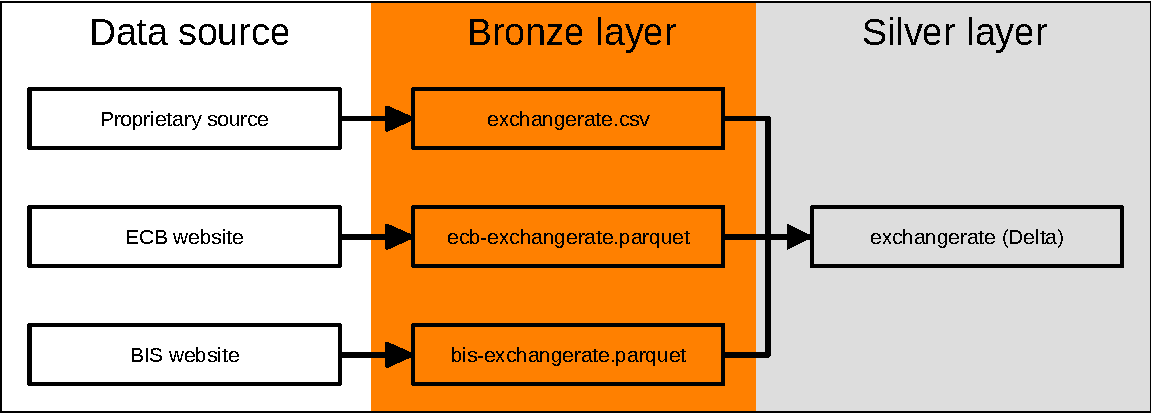
\includegraphics[height=5cm]{exchangerate-architecture}
	\caption{Data pipeline of exchange rate data.}
	\label{fig:function_exchangerate}
\end{figure}

Figure \ref{fig:function_exchangerate} illustrates the data pipeline used to generate a clean exchange rate data set. The pipeline consists of the following parts:
%
\begin{itemize}
	\item Download exchange rate data from the ECB's website and store the result in the bronze layer. As suggested in \textcite{Strengholt.2025}, the structure of the data is preserved. However, the downloaded Zip-file is unzipped and the content of the enclosed csv-file is converted into the Parquet file format. The archive itself is fetched and unpacked in a temporary directory on the local disk of the driver, so that only the resulting Parquet file ever reaches the data lake. This matters in a cloud deployment, where the Bronze layer is an object store volume that should not be burdened with files that are deleted again moments later.
	\item Optional: Download exchange rate data from the BIS's website and store the result in the bronze layer, following the same procedure as for the ECB data. Note that the BIS quotes its bulk exchange rate statistics against the US dollar and reports average rather than reference rates. The pipeline therefore converts these quotes into euro terms using the ECB's EUR/USD reference rate of the same day before the sources are combined, and drops the days for which the ECB does not provide such a rate.
	\item Optional: Download exchange rate data from a commercial data provider and transform it into the structure described in the annex document \emph{Annex - Exchange Rates - Data Dictionary.xlsx}. Save the result as the CSV file \verb|exchangerate.csv| in the Bronze layer as specified in the directory tree in figure \ref{fig:dirstruct_exchangerate}. The CSV file format was chosen, because it allows to impose a schema, which allows for better data validation and contributes to more stability. The schema is declared in the module, since this is the one source whose shape the pipeline does not learn from the file a publisher sent, and the columns of the file therefore have to be the ones of the annex document and in its order. Nothing in the module writes into that folder; the file is placed there by whoever maintains the quotes, as in the entity master data and the market price data modules.

	The file is checked before it is combined, and refused as a whole where a row would be misread: a reference date not written as \verb|YYYY-MM-DD|, a base currency other than the euro, a rate that is missing or not positive, or one day and currency pair quoted twice. The first of these matters most. The combination compares reference dates as text -- to find the date every source reaches, to cut the sources back to it, and to decide which source wins a day -- so a date written differently from the ECB's is not the same day to it. Without the check, a single row dated \verb|2020-10-5| beside ECB rates reaching 31 December would cut the whole table, every currency, back to 6 October, because \verb|2020-10-5| sorts before \verb|2020-10-06| as text, and leave two days with two rates each.
	\item Combine the data sets in the Bronze layer. Only use data up to the latest date in the data set in the least up-to-date sample. This should ensure that the exchange rate data set is always complete.
	\item Clean the data to avoid duplicated values. Where more than one source quotes the same currency pair on the same day, the \emph{fincommons} Python package prefers proprietary data over ECB data over BIS data, and only the winning quote is carried forward. The precedence is expressed as an explicit rank of the sources rather than as an ordering of the combined table, because the order in which the rows of a union arrive is not guaranteed and a rule that relies on it would silently change with the query plan.
	\item Fill the days on which no source quotes -- weekends, holidays and the gaps a source leaves behind -- with the last rate quoted on or before that day, so that the resulting data set holds one row per calendar day and currency pair. The fill follows the time series of the currency pair rather than that of an individual source, since the quote that closes a gap need not come from the source that opened it. Filling each source separately would leave a hole wherever the sources alternate, and an amount dated in such a hole would convert to nothing. The fill stops at the last quote of a pair rather than running on to the cutoff date, and days before the first quote of a pair are not filled either: a currency that ceases to be quoted ends with its last observation instead of carrying a stale rate forward indefinitely.

	Which rows are filled is recorded in the column \verb|IMPUTED|, which is true on a day whose rate was carried from an earlier quote and false on a day a source quoted. Wherever the ECB is the source, the imputed days are the weekends and the TARGET closing days, on which it does not publish; any other day without a quote is marked as well, whatever the reason for the gap, since a carried rate is imputed either way. A quote a source makes on a weekend is not imputed, and a re-based cross rate is imputed where either of the two euro rates it is computed from is. The column lets an analysis restrict itself to quoted rates, or see how much of a result rests on carried ones.
	\item Where an organisation does not have the euro as its national currency, data engineers can re-base the data so that the resulting data set contains exchange rates that correspond to the domestic currency. This is achieved via the transformation
	$$P^{other/domestic}_t = \frac{P^{other/EUR}_t}{P^{domestic/EUR}_t}.$$
	The transformation is applied to the combined data set, so that quotes originating from the proprietary source and the BIS are re-based along with those of the ECB. The euro is added as a quoted currency against the new base, while the new base currency is not quoted against itself.
	\item Store the result in directory \verb|exchangerate| in the Silver layer. The structure and content of the resulting data set are described in the annex document \emph{Annex - Exchange Rates - Data Dictionary.xlsx}. Each run recomputes the table in full rather than adding to it.
\end{itemize}

The table is written as Parquet or as Delta, which the update functions take as an argument. Parquet is the default, because it is the format every engine reads without a further dependency, which is what a table meant to be shared should be. Delta is worth asking for where the table may be queried while it is rebuilt: a Delta update replaces it in a single transaction, so that a reader sees either the previous version in full or the new one and never a half-written file, and the previous versions remain readable. A Parquet update deletes the table before it writes the new one, which leaves a window in which a reader finds it missing. The table is read back in whichever of the two formats it is stored in, so the choice does not have to be repeated when it is queried, and switching an existing table from Parquet to Delta means deleting the directory first, since Delta will not adopt Parquet files it has no transaction log for.

Figure \ref{fig:dirstruct_exchangerate} shows the directory structure that is used for the implementation of this pipeline.

% Directory tree
\begin{figure}[h!]
	\centering
	\begin{subfigure}[t]{.48\textwidth}
		\centering
		\begin{forest}
			for tree={
				%font=\ttfamily,
				grow'=0,
				child anchor=west,
				parent anchor=south,
				anchor=west,
				calign=first,
				edge path={
					\noexpand\path [draw, \forestoption{edge}]
					(!u.south west) +(7.5pt,0) |- node[fill,inner sep=1.25pt] {} (.child anchor)\forestoption{edge label};
				},
				before typesetting nodes={
					if n=1
					{insert before={[,phantom]}}
					{}
				},
				fit=band,
				before computing xy={l=15pt},
			}
			[bronze
			[exchangerate
			[ecb
			[ecb-exchangerate.parquet]
			]
			[bis
			[bis-exchangerate.parquet]
			]
			[internal
			[exchangerate.csv]
			]
			]
			]
		\end{forest}
		\caption{Bronze layer.}
	\end{subfigure} %
	~
	\begin{subfigure}[t]{.48\textwidth}
		\centering
		\begin{forest}
			for tree={
				%font=\ttfamily,
				grow'=0,
				child anchor=west,
				parent anchor=south,
				anchor=west,
				calign=first,
				edge path={
					\noexpand\path [draw, \forestoption{edge}]
					(!u.south west) +(7.5pt,0) |- node[fill,inner sep=1.25pt] {} (.child anchor)\forestoption{edge label};
				},
				before typesetting nodes={
					if n=1
					{insert before={[,phantom]}}
					{}
				},
				fit=band,
				before computing xy={l=15pt},
			}
			[silver
			[exchangerate
			[exchangerate]
			]
			[...]
			]
		\end{forest}
		\caption{Silver layer.}
	\end{subfigure}
	\caption{Directory structures for exchange rate data. In the Silver layer, \emph{exchangerate} is the directory of a table and not a single file.\label{fig:dirstruct_exchangerate}}
\end{figure}

Module \emph{exchangerate} of the \emph{fincommons} Python package contains the functions to perform the data processing steps described above. It is organised along the layers of the pipeline: one part declares the layout of the data lake and the schema of the proprietary source, a second downloads the public reference rates into the Bronze layer, and a third combines them into the Silver layer. The Silver layer part also provides the function \verb|convert2ccy|, with which data scientists convert a column of monetary amounts into a target currency. It is the reason why the Silver table is kept at a calendar-day grain: an amount agreed on a weekend still has to be converted, and a table that only held the quoted business days would leave such amounts unconverted. Amounts whose currency is already the target currency pass through at a rate of one, while amounts in a currency that the data set does not cover on the given date receive neither a rate nor a converted value, so that the absence of a quote remains visible instead of being silently approximated. The conversion itself runs on Spark, but the function accepts a Spark, pandas or polars data frame and returns the same kind of frame it was given, so a data scientist working on a sample in pandas does not have to move it into Spark first. Amounts are matched to rates by calendar day, so an amount dated with a time of day is converted at the rate of its day.

A run of the pipeline consists of the two downloads, of which the BIS one is optional, and the Silver layer update, which takes the target format, whether the BIS quotes are to be used and the currency to re-base to. The function \verb|update_exchangerate| runs all of them in one call and passes those arguments on. While it combines the sources it reports the last date each of them reaches together with the cutoff taken from them, because which source is holding the table back is the question a reader of the log asks. Further documentation on the module's functionality can be found in its README file.


\chapter{Entity master data} \label{ch:entitymasterdata}


% General motivation
Under current European reporting regimes such as EMIR or SFTR the identification of individual counterparties is based on the Legal Entity Identifier (LEI). The LEI is a string of twenty seemingly random alphanumeric values with no immediately recognisable meaning unless it is augmented with further reference data. This includes, among others, the name, country or sector of an entity. Although  some reference data such as sector and country of a counterparty is also reported under EMIR and SFTR, there are several analytical use cases, which benefit from a well-curated entity master data set. This pertains mostly to the calculation of group-specific market indicators such as aggregates based on countries, sectors or business models, which is a necessary data processing step for the generation of dashboards and market reports. To facilitate such analyses, the \emph{fincommons} Python package includes functions for the creation of such an entity master data set.

\begin{figure}[h]
	\centering
	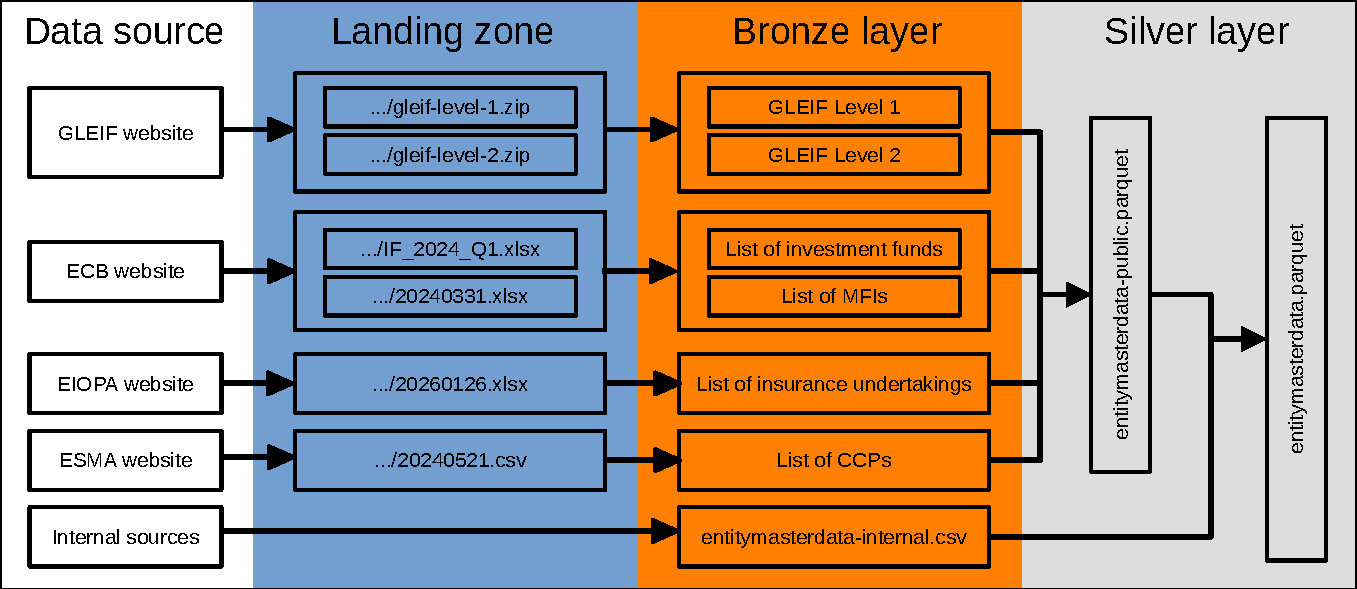
\includegraphics[height=6cm]{entity-master-data-architecture}
	\caption{Data pipeline of entity master data.\label{fig:function_entitymasterdata}}
\end{figure}

% General implementation
Within the \emph{fincommons} framework, the creation of an entity master data set follows \textcite{ESMA.2018} and \textcite{Lenoci.2021}.\footnote{More recently, also see \textcite{Pezzini.2024}.} The corresponding data pipeline is shown in figure \ref{fig:function_entitymasterdata} and consists of the following steps:
%
\begin{itemize}
	\item Load data from various public sources (ECB, EIOPA, ESMA, GLEIF) into the respective folders of the landing zone. GLEIF describes who an entity is and how it is related to other entities, and the sectoral registers state what it does: the ECB lists of investment funds and of monetary financial institutions, the EIOPA registers of insurance undertakings and of institutions for occupational retirement provision (IORPs), and the ESMA list of central counterparties. Between them they fill the field SECTOR, whose values are listed in table \ref{tab:entitymasterdata-sector}.\footnote{The target folders are listed in the module's README file.} Two of these are downloaded by the package. The GLEIF golden copies are fetched from a link that has to be given to the download, because GLEIF publishes no stable address for the most recent release and changes it with every one of them. The list of central counterparties is taken from a public GitHub repository that keeps the information in machine-readable form, since ESMA publishes its registers of authorised and of recognised counterparties as pdf files, which cannot reasonably be read. The ECB and EIOPA registers cannot be reached through a standardised interface at all and have to be placed in the landing zone by hand, under the names the module's README file states, from which the reference date of the register is read.

A download leaves the register or nothing. The answer is written under a temporary name and put in place only once it is complete, so an interrupted download leaves nothing behind under the name the Bronze import reads. An error answer, and an answer that is served with a success status but does not open as the archive it should be, are refused for the same reason: a GLEIF link that has gone stale answers with an error page, which would otherwise be stored under the name of the register and imported as if it were one.
	\item The registers are imported into the Bronze layer to make them queryable. This entails that the data is converted to Parquet from the formats the publishers use: the GLEIF golden copies are read from the zipped CSV files that GLEIF publishes alongside its XML ones, the ECB and EIOPA registers from the Excel workbooks they are handed out as, and the list of CCPs from a CSV file. No major changes to the schema are made so that all potentially useful information remains available.
	\item Optional: Prepare internal entity master data so that it conforms to the structure described in the annex document \emph{Annex - Entity Master Data - Data Dictionary.xlsx}. This data could be obtained from supervisory or proprietary sources as in, e.g., \textcite{Lenoci.2021}. Save the result as a CSV-file in the Bronze layer as specified in the directory tree in figure \ref{fig:dirstruct_entitymasterdata}. The CSV file format was chosen, because it allows to impose a schema, which supports data validation and contributes to greater stability of the data pipeline. The file is checked before it is combined with anything: a file without the field LEI, one with a field the entity master data set does not have, and one that describes the same LEI twice are refused, because the first would displace nothing, the second would lose what it says under the unknown field when the table is written, and the third would leave the choice between the two descriptions to the order in which Spark happens to read them. An LEI that does not have the form of one is kept and named in a warning.
	\item In case internal data is used, the public and internal data sets are combined and de-duplicated. The current implementation of \emph{fincommons} prefers internal data over public data. Thus, data engineers should ensure that when internal data is used, it is \emph{at least} of the same quality than the public data. This is because the processing function only keeps the internal information when there are duplicated values in the merged data set.\footnote{One approach to achieve this is to build on the public data set and enrich it with internal information before saving in the Bronze layer from where it is combined with the public data again. Although this leads to computational redundancies, it ensures that the \emph{fincommons} code base can be used within any organisation to produce the best internationally harmonised entity master data set}.
	\item Add two catch-all entities, which serve at later stages of a data processing pipeline. The entity ``Other'' collects what an aggregation does not show on its own -- the reporting counterparties below the top fifteen of the data quality monitoring of EMIR and SFTR are filed under it, for example, and a chart whose legend names the top five categories puts the rest there -- and the entity ``Unknown'' takes what could not be identified at all, which makes data quality issues easy to spot. The package adds both to the entity master data set itself, under the LEIs \verb|XOTHERX0000000000064| and \verb|XUNKNOWNX00000000025|. Both have the form ISO 17442 prescribes, so that they pass every check an LEI is put to: eighteen characters, padded with zeros, followed by two check digits that make the whole number leave a remainder of one on division by 97. The first four characters of an LEI name the Local Operating Unit that issued it, and none has issued one under \verb|XOTH| or \verb|XUNK|: of the 3,424,918 LEIs of the GLEIF golden copy of 8 September 2026, 521 begin with an X and none with either prefix. A proprietary list that describes one of the two, with a sector of its own for instance, takes precedence over the package's description as it does for any other entity.
\end{itemize}


% Sector codes
\begin{table}[h]
	\centering
	\begin{tabular}{l l l p{6.2cm}}
		\hline
		SECTOR & Rank & Register & Content \\
		\hline
		\verb|CCP|  & 1 & ESMA   & \raggedright Central counterparty. The field SUBSECTOR distinguishes an authorised EU counterparty (\verb|EUCCP|) from a recognised third country one (\verb|T1CCP|, \verb|T2CCP|). \tabularnewline
		\verb|INUN| & 2 & EIOPA  & Insurance undertaking. \\
		\verb|ORPI| & 3 & EIOPA  & Institution for occupational retirement provision. \\
		\verb|CB|   & 4 & ECB    & Central bank. \\
		\verb|CDTI| & 4 & ECB    & Credit institution. \\
		\verb|OFI|  & 4 & ECB    & Other institution on the list of monetary financial institutions. \\
		\verb|MMF|  & 4 & ECB    & Money market fund. \\
		\verb|UCIT| & 5 & ECB    & Investment fund compliant with the UCITS directive. \\
		\verb|AIFD| & 5 & ECB    & Alternative investment fund. \\
		\verb|INVF| & 5 & ECB    & Investment fund the register reports neither of the two about. \\
		\hline
	\end{tabular}
	\caption{Values of the field SECTOR, with the register each is taken from and the rank that settles which one is kept where an entity stands in more than one of them.\label{tab:entitymasterdata-sector}}
\end{table}

An entity can appear in several of these registers, and the rank in table \ref{tab:entitymasterdata-sector} decides which description is kept. The ordering is by how much the register says: a central counterparty is licensed as a credit institution in a number of member states and would otherwise carry that description, and a money market fund stands on the list of investment funds as well. Two of the ranks deserve a word. The insurance register is placed above the register of institutions for occupational retirement provision because a number of entities stand in both -- the Pensionskassen constituted as insurers among them -- and the insurance register states the authorisation the entity holds, whereas the IORP register states an activity carried on under it. The four values the list of monetary financial institutions supplies share one rank, and so do the three the list of investment funds supplies, since each set comes from one register and is mutually exclusive within it. A register can also carry the same LEI twice -- a central counterparty authorised under more than one heading stands in the list of CCPs once per heading, and an institution licensed in several member states stands in the list of MFIs once per state -- and the rank settles nothing there. The choice therefore runs on through the sector and the subsector, preferring a row that states one to a row that does not and otherwise taking the alphabetical one. That decides nothing anyone asked about, but it decides it the same way on every run, which is what the table has to do to be comparable with itself. The three fund codes are read off what the register says about compliance with the UCITS directive; the field IF\_UCITS\_COMPL keeps that statement itself, which is not the same thing as the sector, and SUBSECTOR carries the investment policy the fund pursues.

All of this rests on the LEI being written the same way in every register, since the registers are joined on it as text and an LEI written differently is a different key: it matches no entity of the GLEIF data, and the entity it stands for goes without the sector the register would have given it. The registers do not always write it the same way. The ECB and EIOPA registers are converted from spreadsheets by hand and the list of central counterparties is compiled from ESMA's pdf files, and in September 2026 the list of central counterparties carried six LEIs with a trailing space and the IORP register three in lower case. Joined as they stand, they leave two central counterparties, KDPW\_CCP and Euronext Clearing Athens, and three Italian pension funds without a sector, and with them their positions in every sector aggregate of the EMIR and SFTR data. Every LEI is therefore written the way GLEIF writes it before it is joined -- blanks, including the non-breaking space a spreadsheet leaves, removed and letters put in upper case -- in the registers, in the GLEIF data itself and in a proprietary list alike. Since an LEI contains neither blanks nor lower-case letters, this changes no LEI that was well-formed. One that still does not have the form ISO 17442 gives it, eighteen letters or digits followed by two check digits, is kept but named in a warning together with the register it came from.

Figure \ref{fig:dirstruct_entitymasterdata} shows the directory structure that is used for the implementation of this pipeline. The Silver layer holds two tables addressed by path, \emph{public} for the data set built from the public registers alone and \emph{main} for the one a proprietary list has been put in front of.

Either table can be written as Parquet or as Delta, and the update functions take the choice as an argument. Parquet is the default, because it is the format every engine reads without a further dependency, which is what a table meant to be shared should be. Delta buys two things Parquet does not have and is worth choosing where they matter: a rebuild replaces the table in a single transaction, so that a reader either sees the previous version in full or the new one and never the half-written state that overwriting a set of Parquet files in place would leave behind, and the previous versions of the table remain readable. The table is read back in whichever format it was written in, so the choice does not have to be repeated when it is queried. Switching an existing table from Parquet to Delta is the one direction that needs a hand, since Delta will not adopt Parquet files it has no transaction log for: the directory has to be deleted before the first Delta update.

% Directory tree
\begin{figure}[h!]
	\centering
	\begin{subfigure}[t]{0.32\textwidth}
		\centering
		\begin{forest}
			for tree={
				%font=\ttfamily,
				grow'=0,
				child anchor=west,
				parent anchor=south,
				anchor=west,
				calign=first,
				edge path={
					\noexpand\path [draw, \forestoption{edge}]
					(!u.south west) +(7.5pt,0) |- node[fill,inner sep=1.25pt] {} (.child anchor)\forestoption{edge label};
				},
				before typesetting nodes={
					if n=1
					{insert before={[,phantom]}}
					{}
				},
				fit=band,
				before computing xy={l=15pt},
			}
			[landing
			[ecb
			[investment\_fund
			[IF\_2025\_Q3.xlsx]
			]
			[mfi
			[20250130.xlsx]
			]
			]
			[eiopa
			[insurance\_undertaking
			[20250202.xlsx]
			]
			[iorp
			[20250202.xlsx]
			]
			]
			[esma
			[ccp
			[ccp\_list.csv]
			]
			]
			[gleif
			[level\_1
			[20260202-0800.zip]
			]
			[level\_2
			[20260202-0800.zip]
			]
			]
			]
		\end{forest}
		\caption{Landing zone.}
	\end{subfigure}
	\begin{subfigure}[t]{0.32\textwidth}
		\centering
		\resizebox{\textwidth}{!}{%
		\begin{forest}
			for tree={
				%font=\ttfamily,
				grow'=0,
				child anchor=west,
				parent anchor=south,
				anchor=west,
				calign=first,
				edge path={
					\noexpand\path [draw, \forestoption{edge}]
					(!u.south west) +(7.5pt,0) |- node[fill,inner sep=1.25pt] {} (.child anchor)\forestoption{edge label};
				},
				before typesetting nodes={
					if n=1
					{insert before={[,phantom]}}
					{}
				},
				fit=band,
				before computing xy={l=15pt},
			}
			[bronze
			[ecb
			[investment\_fund
			[2019Q1.parquet]	
			[...]
			[2025Q3.parquet]
			]
			[mfi
			[20260130.parquet]
			]
			]
			[eiopa
			[insurance\_undertaking
			[20260202.parquet]
			]
			[iorp
			[20260202.parquet]
			]
			]
			[esma
			[ccp
			[ccp\_list.parquet]
			]
			]
			[gleif
			[level\_1
			[20260202.parquet]
			]
			[level\_2
			[20260202.parquet]
			]
			]
			[internal
			[entitymasterdata-internal.csv]
			]
			[...]
			]
		\end{forest}
		}
		\caption{Bronze layer.}
	\end{subfigure}
	\begin{subfigure}[t]{0.32\textwidth}
		\centering
		\begin{forest}
			for tree={
				%font=\ttfamily,
				grow'=0,
				child anchor=west,
				parent anchor=south,
				anchor=west,
				calign=first,
				edge path={
					\noexpand\path [draw, \forestoption{edge}]
					(!u.south west) +(7.5pt,0) |- node[fill,inner sep=1.25pt] {} (.child anchor)\forestoption{edge label};
				},
				before typesetting nodes={
					if n=1
					{insert before={[,phantom]}}
					{}
				},
				fit=band,
				before computing xy={l=15pt},
			}
			[silver
			[public
			[\_delta\_log]
			[part-....parquet]
			]
			[main
			[\_delta\_log]
			[part-....parquet]
			]
			]
		\end{forest}
		\caption{Silver layer, written as Delta.}
	\end{subfigure}
	\caption{Directory structures used for entity master data. A Silver table written as Parquet holds the same part files without the transaction log beside them.\label{fig:dirstruct_entitymasterdata}}
\end{figure}

The data processing steps described above are implemented in module \emph{entitymasterdata} of the \emph{fincommons} Python package. Documentation of its functionality and application is found in the README file of the module in the code repository, which also states the names the registers that cannot be downloaded have to be placed under, the reference date being read off the name of the file.



\chapter{FIRDS}\label{ch:firds}

\section{Introduction}

Under Article 27 of of Regulation (EU) No 600/2014 (MiFIR) trading venues shall provide ESMA with identifying reference data pertaining to financial instruments admitted to trading or traded on a trading venue.\footnote{See \url{https://eur-lex.europa.eu/eli/reg/2014/600}.} This data set is commonly referred to as FIRDS data. A list of the reported information is provided in the annexes of the associated RTS.\footnote{See \url{https://eur-lex.europa.eu/eli/reg_del/2017/585}.}


\section{Data pipeline}

The data pipeline of FIRDS data follows the considerations of section \ref{sec:intro-data}. FIRDS-specific aspects are discussed in more detail in the following.

The pipeline stores its data in three formats, and which one a data set is stored in follows from how that data set comes to change rather than from which layer it belongs to. The landing zone holds the files as ESMA publishes them, compressed XML, because it is a place for deliveries and not yet for data. A data set that is only ever added to, one file at a time, and never altered afterwards is stored as plain Parquet; that is the Bronze layer, discussed in section \ref{sec:firds-bronze}. A data set that is changed where it stands, whose rows are closed, replaced and appended to one delivery at a time, is a Delta table, because that is what a transaction log is for: the historical database \emph{main} and the \emph{watermarks} table that records how far it has been built. A data set that is derived in full from another and rebuilt rather than changed loses nothing by having no log, and is therefore Parquet again unless it is asked to be Delta; that is the \emph{compact} table, and the reason one might ask is set out where it is described. Why the transaction log is Delta Lake rather than Apache Iceberg is a decision for the framework as a whole and is argued in section \ref{sec:intro-data-formats}; FIRDS is the module that depends on it most, because its historical database is updated with MERGE statements rather than rewritten.

\subsection{Landing zone}

FIRDS data is hosted by ESMA and publicly available as compressed XML files. Thus, the first stage of the data pipeline is to download data from ESMA's website into the landing zone. The download procedure follows the instructions in the ESMA Guide \emph{FIRDS - Instructions on access and download of full and delta reference data files}.\footnote{Available at \url{https://www.esma.europa.eu/document/firds-instructions-access-and-download-full-and-delta-reference-data-files}.}

Consistent with the ESMA Guide, FULINS data is downloaded only once for a certain date that marks the beginning of the historic database. For periods after the starting date only DLTINS data is downloaded to incrementally update the database.

The folders at the root of each panel of figures \ref{fig:dirstruct_firds_landing_bronze} and \ref{fig:dirstruct_firds_silver_gold} -- \emph{landing}, \emph{bronze}, \emph{silver} and \emph{metadata} -- are the four paths the \emph{firds} section of the configuration file names, and they are the only locations the module takes as given. Everything below them is created by the module itself and is named as shown. An organisation that keeps several sources apart within one data lake would point the configured paths at, say, \emph{/data/landing/esma/firds}, and the folders below them would be the same ones: where the configured paths sit is a decision of the configuration file, and nothing in the module depends on it.

Panel (a) of figure \ref{fig:dirstruct_firds_landing_bronze} illustrates the folder structure of the landing zone. Data downloaded from ESMA's website is stored in the folder \emph{import}. If the import into the Bronze layer is successful, the respective ZIP file is moved into the \emph{finished} folder. If the import fails, the data is moved into the folder \emph{error}.

Which files a run downloads is decided by comparing names: every file of the full sample the history starts from, every delta file published after it and the most recent cancellations file are fetched unless a file of the same name is already in \emph{import} or \emph{finished}. Resuming after the newest delta file in \emph{finished} instead would be correct as long as every file succeeds, but a delta file is often published in several parts, and a part that failed while a later file succeeded would then never be requested again, so that the history would silently lack its records. Comparing names repairs such a gap on the next run, whatever went wrong before, and a file set aside in \emph{error} counts as missing for the same reason. The comparison presupposes that \emph{finished} is kept; it is the record of what the Bronze layer has been built from. A download is written under a temporary name and only renamed once it is complete, an error answer of the server is raised rather than stored, and an archive that does not open is refused, because a truncated file under its final name would count as held and would not be fetched again. The register states an MD5 digest for every file, and a file that does not match it is refused as well.

The register itself is read page by page. It publishes some three thousand files a year, and a single request for ten thousand rows returns an arbitrary part of the list once the period asked about holds more files than that, which happens within about three years, without any sign that something is missing. The pages are sorted so that they follow one another, and a list that ends up shorter than the number of files the register reports is refused. Asking the register about the whole period since the full sample on every run would also make the answer grow without bound, so the landing zone records, in a small file of its own, the last day up to which every part of the full sample and of the delta files has been imported, and the next run asks only from a week before that day on. The week of overlap is there because ESMA sometimes publishes a file after the day it is dated, and such a file is not in the answer the record was computed from. The same file also records which days the register listed a delta file for, so that the Silver layer can tell a day it holds no records for from one that was never published; how far the Silver layer has built the history, which it writes there itself, since the landing zone cannot read a watermark that lives in a Delta table and its own record is written before anything is downloaded and so lags behind; and which days turned up after the history had passed them. The day moves forward only while nothing before it is missing, which keeps a failed file within the window until it has been imported.

\subsection{Bronze layer\label{sec:firds-bronze}}

For further processing, the data in the landing zone must be decompressed. Afterwards, the content of the resulting XML file is parsed and stored in the Bronze layer in the Parquet file format. Since the received XML files can have different schemas, which can also change over time, data with a specific schema is stored in a dedicated directory. Within those directories, data is partitioned based on the date information that is contained in the file name of an XML file. Panel (b) of figure \ref{fig:dirstruct_firds_landing_bronze} illustrates this structure.

That the Bronze layer is plain Parquet and not a Delta table follows from what it is asked to do. Each file of the landing zone is written into it once, as a partition of its own, and nothing that has been written is altered afterwards, so there is no row to update, no version to read back and nothing for a transaction log to reconcile. The directories themselves carry the information the Silver layer needs: the schema a file was published under is the directory it lies in, its reference date is the name of its partition, and an empty partition records that a file was imported and held no records. The Silver layer finds all of this by listing directories, which is as cheap as it is transparent, whereas a Delta table records its partitions in its log and has no way of stating an empty one. Plain Parquet is finally what any reader opens without a further dependency, which suits a layer that serves as the queryable archive of what was delivered.

What is given up is the atomicity of a write, and it is worth stating where the pipeline makes up for it. Spark writes into a temporary directory and moves the files into the partition only once every task has succeeded, so an import that fails usually leaves nothing behind. The move itself is not a single transaction, however, least of all on object storage, and an import that fails during it can leave part of a file in the partition. The file is then set aside in \emph{error}, which the landing zone counts as missing, so it is downloaded and imported again, and its partition may come to hold some records twice. That is harmless because the Silver layer does not rely on the Bronze layer being free of duplicates: exact duplicates are dropped before a delta file is applied, and the history is initialised with one version per instrument from the full file. A file that did arrive in \emph{finished} is not imported a second time. Delta would not have spared the pipeline the problem of schema vintages discussed below either, since it too refuses an append that changes the type of a column, and the change would then have stopped the import rather than the read.

Note that since FULINS data is usually only downloaded once, there should only be one partition in the folder of the corresponding schema -- in the example in figure \ref{fig:dirstruct_firds_landing_bronze}, this means only one sub-folder in folder \emph{auth\_017\_001\_02}. Where there are several, the history is started from the newest of them and the others are passed over with a warning, since a full sample states the reference data in full and an older one only adds instruments the newest one no longer carries.

The current implementation of \emph{fincommons} in general preserves the original schema of the data, however, some header information is currently dropped.\footnote{Metadata management as proposed in \textcite[chapter 6]{Strengholt.2025} is currently considered/in development.}

Storing each schema in a directory of its own solves only half of the problem, because a schema can also change while keeping its name. The schemas the parser reads with are derived from ESMA's XSD files and are stored with the module, and deriving them again can change a type: the money and rate fields can be read as a floating point type under one derivation and as a decimal one under another, and the cancellation element \emph{CancRcrd} as a full reference data record under one and as the reduced one the schema actually states under another. The Bronze layer is append-only and keeps the files it has already written, so a single directory comes to hold files written under two vintages of what is nominally one schema. Parquet does not reconcile them. A reader must state one type per column, and the format refuses to hand a column written as a floating point number to a reader asking for a decimal, so a naive read of the directory fails outright and the daily job stops -- not on the day the schema was changed, but on the first day thereafter on which a new file joins the old ones.

A schema can also change its name, which is the complement of the case just described and is handled by the directory structure rather than despite it. ESMA published the delta file as \emph{auth.036.001.02} until 31 January 2022 and as \emph{auth.036.001.03} from 1 February 2022 onwards, so a history reaching back before that date is built from files of both. Earlier still, up to 21 September 2019, the full and the delta file were published under drafts of their definitions, \emph{DRAFT13auth.017.001.01} and \emph{DRAFT6auth.036.001.01}, and the register still lists them back to 2018. Each definition is given a directory named after it, as every other message is, and the Bronze layer therefore records which message each file was published under rather than obscuring it. What has to span the two is the Silver layer, which asks for the reference dates of both directories together and applies them as the single chronological sequence they form; the change of definition falls on a day boundary and is invisible to the history built across it. Sampling the register one delta file per quarter from 2020 to 2026 found this to be the only such change in that period, and the full file to have carried \emph{auth.017.001.02} throughout, across twenty-seven quarters. The drafts are a change of name and of nothing a record states: scanning the whole full file of 29 December 2018 and a sample of the draft delta files of 2019 found every element path they use in the schema of the definition that replaced them, so they are read with that schema. What does differ is their timestamps, which state no time zone -- \emph{2019-01-02T08:00:00} where a later file states \emph{2019-09-23T08:43:16Z} -- and which Spark would read in the time zone of the session. A session set to Vienna turns that first trading time into 07:00 UTC and moves a termination at midnight to the day before, so the drafts are read in UTC whatever the session says. They also do not state the relevant trading venue, which is empty for the records they carry. A file whose message the parser does not recognise is not guessed at: it is set aside in the \emph{error} folder and the definition it states is named in the log, so a further change announces itself rather than corrupting the history.

The read that builds the historical database is therefore arranged so that the vintage of a file cannot matter. It proceeds partition by partition rather than over the whole directory, so that the files it has to reconcile are those of a single publication day. Within a partition it groups the files by the types they state for the fields the pipeline actually reads and reads each group on its own, which is the one case that genuinely requires separate reads. It asks for the paths the translation to the analytics schema reads and for nothing else, which means that a change in a field the pipeline never uses -- the great majority of the schema, which describes derivative attributes in considerable detail -- passes unnoticed and costs nothing. Finally it casts every field it read to the type the historical database carries, so that what the history is built from has one fixed schema whatever the partition held. The types chosen for that final cast are those the historical database carries, and the schema of that database is derived from them rather than stated a second time, so that the two cannot drift apart.

Reading only the paths the pipeline uses protects it against changes elsewhere in the schema, but it is worth being precise about what that protection does not extend to. A path the pipeline does use may be absent from a record not because the source stopped stating it but because the source states it somewhere else, and under a declared schema the two are indistinguishable: an element the reader did not ask for and an element the file did not contain both arrive as an empty value. The publication period of a record is the case in point. \emph{TechAttrbts/PblctnPrd} is a choice in the ISO 20022 sense, and ESMA exercises it differently according to what the record reports. In the delta file of 5 January 2020, the 32,875 records reported as new or modified state the open-ended form \emph{FrDt}, whereas of the 24,107 terminations 19,630 state the closed range \emph{FrDtToDt} and the remaining 4,477 state no publication period at all, carrying nothing in \emph{TechAttrbts} beyond the competent authority and the trading venue.

Reading the first branch alone leaves every termination without a validity date, and the consequence is silent. The date on which a superseded version is closed is the day before the incoming record begins, so where the incoming date is empty the closing date is empty too and the version it should have closed remains in force. Nothing fails at the time. The history goes on being built, the latest-record flag becomes ambiguous, and in a history built that way, after five delta files 132,977 instruments carried as many as eight versions in force each. The fault surfaces only when a MERGE matches several source rows against one target row and refuses to proceed -- an error naming the merge rather than the record that caused it, and five days removed from it. The pipeline therefore reads every branch of the choice and takes the reference date of the file for a termination that states no period, as it does for a cancellation for the same reason; the history built so from the same nine delta files holds 17.7 rather than 15.6 million versions, with the number of versions in force exactly equal to the number of latest records. The pipeline also refuses a record whose publication period it cannot read, so that a branch not yet accounted for stops the run where the record enters rather than days later somewhere else. The general point is taken up in section \ref{sec:intro-data-schema}.

That leaves the question of which types the database should carry, which is a question about the data and not about how a file is read. Four of the fields are money or rates: the total issued nominal amount, the nominal value per unit, the fixed interest rate and the price multiplier. Double precision floating point is the natural reading of a numeric XML element and the wrong one here. A binary floating point number cannot represent a decimal fraction exactly, so a coupon reported as 3.7 per cent would be stored as 0.036999999999999998 and an amount would only ever be as exact as fifteen significant digits allow. For a supervisory record the precision is not an artefact of the arithmetic but part of what the record states, and the XSD files say so explicitly: each of these elements is an \emph{xs:decimal} with a stated number of total and fractional digits. The database therefore carries them as decimals of exactly those precisions.

% Directory tree
\begin{figure}[h]
	\centering
	\begin{subfigure}[t]{0.48\textwidth}
		\centering
		\begin{forest}
			for tree={
				%font=\ttfamily,
				grow'=0,
				child anchor=west,
				parent anchor=south,
				anchor=west,
				calign=first,
				edge path={
					\noexpand\path [draw, \forestoption{edge}]
					(!u.south west) +(7.5pt,0) |- node[fill,inner sep=1.25pt] {} (.child anchor)\forestoption{edge label};
				},
				before typesetting nodes={
					if n=1
					{insert before={[,phantom]}}
					{}
				},
				fit=band,
				before computing xy={l=15pt},
			}
			[landing
				[error
					[...]
				]
				[finished
					[FULINS\_C\_20260103\_01of01.zip]
					[...]
					[FULINS\_S\_20260103\_05of05.zip]
					[DLTINS\_20260104\_01of01.zip]
					[DLTINS\_20260105\_01of01.zip]
					[FULCAN\_20260106\_01of02.zip]
					[FULCAN\_20260106\_02of02.zip]
				]
				[import
					[DLTINS\_20260106\_01of01.zip]
					[...]
				]
			]
		\end{forest}
		\caption{Landing zone.}
	\end{subfigure}
	\begin{subfigure}[t]{0.48\textwidth}
		\centering
		\begin{forest}
			for tree={
				%font=\ttfamily,
				grow'=0,
				child anchor=west,
				parent anchor=south,
				anchor=west,
				calign=first,
				edge path={
					\noexpand\path [draw, \forestoption{edge}]
					(!u.south west) +(7.5pt,0) |- node[fill,inner sep=1.25pt] {} (.child anchor)\forestoption{edge label};
				},
				before typesetting nodes={
					if n=1
					{insert before={[,phantom]}}
					{}
				},
				fit=band,
				before computing xy={l=15pt},
			}
			[bronze
				[DRAFT13auth\_017\_001\_01
					[...]
				]
				[auth\_017\_001\_02
					[{DATADT=2026-01-03}]
				]
				[DRAFT6auth\_036\_001\_01
					[...]
				]
				[auth\_036\_001\_02
					[...]
				]
				[auth\_036\_001\_03
					[{DATADT=2026-01-04}]
					[{DATADT=2026-01-05}]
				]
				[auth\_102\_001\_01
					[{DATADT=2026-01-06}]
				]
			]
		\end{forest}
		\caption{Bronze layer.}
	\end{subfigure}
	\caption{Directory structure for FIRDS data.\label{fig:dirstruct_firds_landing_bronze}}
\end{figure}


\subsection{Silver layer}

The Silver layer consists of two data sets. First, a table named \emph{main}, which is the implementation of the historical database as described in section 4.2 of ESMA's Guide mentioned above.

Due to the use of incremental updates of the \emph{main} table, Delta Tables are used for the implementation. A delta file is applied in two steps against the table. A single MERGE operation changes the versions that the file affects: the versions that the incoming records supersede are closed on the day before the incoming record takes effect and lose their latest-record flag, and a version that was terminated in the ordinary way is replaced by the incoming record. The remaining incoming records are then appended. Both changes address the version in force of an instrument, and an instrument is subject to at most one of them, because only the first record a file carries for an instrument meets the version that was in force before the file. They can therefore be applied together, which matters because each MERGE reads the target table, and a second one would traverse it again only to reach a set of rows the first one did not touch.

Both steps are planned from one fixed version of the table, the one before the MERGE, which is read by its version number. This is not a matter of style. Spark computes the plan again for the append, since the MERGE does not fill the cache the plan is kept in, and a read of the table that is not pinned then sees the table as the MERGE left it. A version the MERGE has just replaced is no longer in force there, so the record that replaced it would be planned a second time as an insertion and appear twice in the history. That would happen whenever a delta file terminates an instrument in the ordinary way and changes it again in the same file.

The implementation departs from the Guide in two respects, both of which follow from the rule that an instrument has one version in force at a time. First, records for the same instrument within one file are chained, each valid until the day before the next one begins, but records that begin on the same day cannot be chained without producing a version that ends before it begins. Of such records only the last in the order new, modified, cancelled, terminated is kept, and exact duplicates are dropped beforehand. For the same reason a record that begins on the same day as the version in force replaces that version rather than closing it, which is what the Guide prescribes for an ordinary termination; following the Guide literally would close the version on the day before it began and leave a version valid on no day at all. Second, what a record does is decided by the version in force rather than by the element it was reported in. The Guide does not describe a record reported as new for an instrument that already exists, since a new instrument is not supposed to exist already, but ESMA reports one when an instrument is admitted again after it was terminated -- a termination remains in force, because it carries no closing date. Inserting such a record would leave the instrument with two versions in force, and the next delta file touching it would match the MERGE against both rows at once and stop the update with an error until the table was repaired by hand. It therefore supersedes the version in force like any other record.

The \emph{main} table is not partitioned. It is instead clustered by the pair of ISIN and MIC code that identifies an instrument on a trading venue, i.e. by the same columns the MERGE matches on. Partitioning the table by the MIC code of the trading venue, on the assumption that this would speed up updates and joins through better opportunities for parallelisation, does the opposite, as measurement shows, and the reasons are general enough to be worth stating in section \ref{sec:intro-data-layout} rather than only here: the partitions are far too small to carry the fixed cost of a partition, the pruning they promise never materialises because a delta file touches most trading venues at once, and, most damagingly, each append writes a separate file for every combination of writing task and trading venue, so that a single day of delta files can arrive as several thousand files of a few kilobytes each. Partitioned that way, the table grew to more than 19,000 files averaging some 16 kilobytes after only three days of updates, and the scan of the versions in force that every subsequent update performs took 27 seconds where the same data in a compacted layout took a little over one. Since that cost grows with the number of files accumulated so far, a backfill over a longer history degrades quadratically. Clustering keeps the columns of the MERGE condition together within files without cutting the table into directories, so that the file statistics can exclude a file from a scan, and the periodic OPTIMIZE that maintains the clustering is incremental: it processes the files that have arrived since it last ran rather than rewriting the whole history.

Clustering alone does not stop the daily MERGE from rewriting the history. Without further provision Delta rewrites every file a MERGE touches in full, and since a delta file concerns instruments all over the table, every file is touched. Re-applying the delta files of two days to a copy of the history of 17 million versions built from the full sample of 5 September 2026 made this visible: the file of 7 September changed 172 versions and copied the other 16,963,552 rows, taking 54 seconds, and the file of 8 September changed 1,180,246 versions and took 85 seconds. The table therefore carries deletion vectors. With them the MERGE records the superseded rows in a small side file and writes only the new versions, and the same two files took 15 and 55 seconds without copying a single row. The distinction matters more than the figures suggest, because without deletion vectors the cost grows with the history, which only grows, whereas with them it follows the size of the delta file. The files written since the previous run are clustered once a week, on the delta file of each Friday, and that OPTIMIZE also rewrites the files in which deleted rows have accumulated, which is most of the table: measured on the same history it took 87 seconds and rewrote all 17 million rows. The weekly cost therefore follows the size of the history rather than the week, so what deletion vectors take off the daily path they put back once a week -- a seventh of the rewrites, which is what makes the trade worth making. The price is a higher reader version of the table, so that a reader outside Spark needs support for deletion vectors; the \emph{compact} table remains the one intended for such readers. The join of a delta file against the versions in force, which Spark cannot broadcast in the form it is written, is not where the time goes: measured, that scan took between 4 and 8 seconds regardless of the size of the file, and restricting it to the instruments of the file made no difference.

Built under the clustered layout, the same three days of history occupy ten files rather than 19,415, and 145 rather than 473 megabytes on disk, with the same number of records. The reduction in size is not a saving from discarding anything but a consequence of the file count itself: every Parquet file repeats a footer, a schema and its dictionary pages, and compression works considerably better across fourteen megabytes of clustered records than across fragments of sixteen kilobytes. A table consisting of very many small files is therefore not merely slow to read, it also occupies several times the space its contents require.

The layout is declared by a function of its own, \verb|declare_silver_main_layout|, which the update calls when it creates the historical database. Its statements are idempotent, so it can be called again on a database that already carries the layout. Declaring deletion vectors upgrades the reader version of the table, which Delta does not undo by itself, and a reader outside Spark then needs support for deletion vectors.

Everything in the Silver layer is derived from the Bronze layer and can be reconstructed from it at any time, which is the reason the Bronze layer keeps the delta files in the first place and a property worth preserving when the pipeline is extended.

Since a delta file only states what changed since the previous one, the files must be applied in chronological order and exactly once. Applying a file twice would attribute wrong validity periods to the affected versions. The pipeline therefore maintains a watermark, i.e. the reference date up to which the historical database has been built, and processes only the files that are newer than it. The watermark is held in a small Delta table named \emph{watermarks} in the metadata area of the data lake, which contains one row per table of the Silver layer and is shown in panel (b) of figure \ref{fig:dirstruct_firds_silver_gold}. Storing it as a path-addressed Delta table rather than, for instance, in a local database file means that the same code serves a workstation and a cluster, where the driver's local filesystem is not a place in which a pipeline should record state. Where an existing historical database carries no watermark, the update is refused rather than restarted from an assumed date, since a wrong assumption would silently corrupt the validity periods.

The watermark is written after the records, and the MERGE and the append are separate commits, so a run can end with a delta file applied only in part. Starting that file again from the table as it then stands would close the versions it had just inserted. Each of the two commits therefore carries the reference date in the commit metadata of the Delta table. A run that finds the append of a date already committed only records the watermark. A run that finds only the MERGE committed plans the file from the version of the table before that MERGE and makes the append alone. Only the commits since the table was last written from scratch are consulted, so a history rebuilt from the Bronze layer does not inherit the marks of the one it replaced. Delta's own mechanism for idempotent writes is not used for this, because the application versions it records survive such a rebuild and would silently suppress every append of the new history.

A history this module built can also say for itself how far it has been built. The commits described above name the reference date they applied, and where the watermark is missing it is recovered from them, with a warning, instead of the database having to be built again. That is the state a run leaves behind when it dies after writing the history and before writing the watermark. A database that carries no such commits is refused.

A reference date is applied only once every part of its delta file has been imported, which the pipeline checks against the names in the \emph{finished} folder of the landing zone; the full sample is checked the same way before the history is initialised. The first incomplete date stops the update: the dates before it are applied, and the run fails naming the missing parts. Carrying on past it would move the watermark beyond the incomplete date, and the records of its missing parts could never be applied afterwards. For the full sample, the names that arrived are not enough on their own. It is published in parts per first letter of the CFI code, and a part that arrived states how many parts its letter has, so a missing part of a letter is noticed; but a letter of which no part at all arrived leaves no trace among the others, and the history would be initialised without that asset class, whose instruments would then reach it only as delta files happened to change them. The landing zone therefore records the names of the parts the register lists for the full sample, and the history is not initialised until every one of them is in the \emph{finished} folder. A data lake filled by hand carries no such list and is initialised from the parts that arrived, with a warning that the check could not be made.

Which dates are considered at all cannot be read off the Bronze layer alone. A day whose delta file was quarantined has no partition there, and a day that was never fetched leaves no trace in the data lake whatsoever, so the candidates are collected from the Bronze partitions, from the file names in the \emph{finished} and \emph{error} folders, and from the days the landing zone recorded the register as having listed. Taking them from the Bronze layer alone would apply the day after a failed one, moving the watermark past records that could then never be applied.

Three states are told apart where a date has no Bronze partition. Parts that were never imported stop the update, as above. A partition that has gone missing although every part was imported stops it as well, and says so differently. A file that carried no records at all is neither: the Bronze layer creates its partition as an empty directory to record that the date was imported and held nothing, and the update passes the date with a warning instead of stopping on it for ever.

Two properties of an incoming record are checked before anything is written, for the same reason the publication period is: the fault they describe does not fail at the time it is made, and a history that goes on building around it costs more to repair than a run that stops on it. The first is that the record says which instrument it is about. An instrument is the pair of ISIN and MIC code, and every comparison the algorithm makes on it is an equality, which no null satisfies, so a record missing either half is never found to supersede anything and is inserted afresh by every file that carries it: the instrument acquires one version in force per delivery, all of them flagged as the latest record, and the compact table counts it once per version. The second is that the record does not begin before the version in force for its instrument. Paragraph 27.b.ii closes that version on the day preceding the start of the incoming record, which prescribes what to do on the assumption that the incoming record starts later; where it starts earlier the arithmetic is still well defined and closes the superseded version before its own start date, so that the version is valid on no day at all and a point-in-time query returns, for every subsequent day, the older record. Both are refused naming the records concerned.

A day whose delta file ESMA publishes after the history has been built past it is the one case the ordering cannot repair. Its records are not in the history, and applying the days after it does not put them there, so the landing zone records the day and the update refuses to continue, naming it. The history can then be rebuilt from that day, or the gap accepted deliberately, after which the update carries on. Every refusal of this kind stops the daily job until someone acts, which is the intended behaviour for a database whose value lies in being complete; where a file is broken at the source and will never arrive, moving the watermark past the day by hand is what lets the history continue, at the price of that day's records.

Second, since securities can be traded on multiple trading venues, FIRDS data in the \emph{main} table can contain multiple observations per ISIN. This can lead to unwanted data explosions when the table is joined with other data sets. To address this, table \emph{compact} is generated, which contains only one row per ISIN. Text fields are concatenated, if multiple entries are available in \emph{main}. The maturity date, the expiry date and the price multiplier keep their types: they hold the value the trading venues agree on and are empty where the venues disagree, since two dates cannot be joined into one date. A cancelled record is left out. The history records it as the version in force of its instrument and venue, as the Guide prescribes, but it states nothing about the instrument, and what it says is that the instrument was never admitted to that venue; counted, it would list the venue among those the instrument trades on, as it would for two ISINs in the history of September 2026. An ISIN whose every venue was cancelled consequently leaves the table altogether, which is the same statement one row further out. Joining the dates as text and parsing the result would, under the strict parsing Spark 4 applies by default, make the whole rebuild fail as soon as a single ISIN carries two different maturities. The values of a text field are sorted before they are concatenated, so that the string an ISIN carries follows from the set of values rather than from the order in which a hash set happens to iterate over them: the aggregation defines no order, the table is rebuilt in full on every run, and without sorting a venue added to an ISIN can appear anywhere in the string rather than beside the others, so that two data lakes holding identical rows need not spell the column identically. A venue that states nothing, finally, is not a venue that disagrees -- a null is omitted, so the value of one venue stands for an ISIN the others are silent about -- and where no venue states a value at all the field is empty rather than an empty string, which is what concatenating an empty list yields; the typed columns are empty in that situation as well, and a reader should not have to distinguish \verb|NULL| from \verb|''| to ask the same question of two columns of one table. Unlike \emph{main}, the \emph{compact} table is not updated incrementally but rebuilt in full from \emph{main} whenever the historical database has changed. It is stored as plain Parquet by default, since it is the table meant to be handed on to analysis and Parquet is what every engine reads without a further dependency, but it can be asked to be a Delta table instead. The reason to ask is not incremental updating but the atomicity of the rebuild: overwriting a plain Parquet data set deletes it before the new one is written and therefore exposes a window in which a reader finds the table missing or only partly written, whereas the Delta write replaces it in a single transaction. That is worth having where the table may be queried while it is rebuilt. A table that already stands keeps the format it is stored in, and requesting the other one is refused rather than carried out: overwriting a Delta table as Parquet deletes its transaction log along with the superseded files, which is not a thing to do as a side effect of naming a format, and in the other direction Delta does not adopt Parquet files for which it holds no log. The directory has to be removed to change the format of a table that exists. How that choice is made is not a question about FIRDS, and the module shares the answer with the other modules whose Silver table is rebuilt in full. Since a Delta table consists of standard Parquet files with a transaction log beside them, and readers for that format are available outside Spark -- the \emph{fincommons} package itself depends on Polars, which reads such tables -- this choice does not compromise the original objective that the data remain accessible to non-Spark software.

The folder structure of the Silver layer is illustrated in panel (a) in figure \ref{fig:dirstruct_firds_silver_gold}.


\subsection{Gold layer}

Currently, there is no data set in the Gold layer, which would be exclusively based on FIRDS data, and the \emph{firds} section of the configuration file accordingly names no Gold path at all. Reference data is an input to the analyses of other data sets rather than the subject of one of its own, so what a Gold layer here would hold is a question that has not arisen yet; the \emph{compact} table of the Silver layer is what those analyses join against.


% Directory tree
\begin{figure}[h]
	\centering
	\begin{subfigure}[t]{0.40\textwidth}
		\centering
		\begin{forest}
			for tree={
				%font=\ttfamily,
				grow'=0,
				child anchor=west,
				parent anchor=south,
				anchor=west,
				calign=first,
				edge path={
					\noexpand\path [draw, \forestoption{edge}]
					(!u.south west) +(7.5pt,0) |- node[fill,inner sep=1.25pt] {} (.child anchor)\forestoption{edge label};
				},
				before typesetting nodes={
					if n=1
					{insert before={[,phantom]}}
					{}
				},
				fit=band,
				before computing xy={l=15pt},
			}
			[silver
				[main
					[\_delta\_log]
					[part-....parquet]
					[deletion\_vector\_....bin]
				]
				[compact]
			]
		\end{forest}
		\caption{Silver Layer.}
	\end{subfigure}
	\hfill
	\begin{subfigure}[t]{0.40\textwidth}
		\centering
		\begin{forest}
			for tree={
				%font=\ttfamily,
				grow'=0,
				child anchor=west,
				parent anchor=south,
				anchor=west,
				calign=first,
				edge path={
					\noexpand\path [draw, \forestoption{edge}]
					(!u.south west) +(7.5pt,0) |- node[fill,inner sep=1.25pt] {} (.child anchor)\forestoption{edge label};
				},
				before typesetting nodes={
					if n=1
					{insert before={[,phantom]}}
					{}
				},
				fit=band,
				before computing xy={l=15pt},
			}
			[metadata
				[watermarks]
			]
		\end{forest}
		\caption{Metadata.}
	\end{subfigure}
	\caption{Directory structure for FIRDS data. The \emph{main} table is not cut into directories: it is clustered, and its files lie beside the transaction log and the deletion vectors. The Delta table \emph{watermarks} in panel (b) records the reference date up to which it has been built.\label{fig:dirstruct_firds_silver_gold}}
\end{figure}






\section{Software architecture}

% Software
Module \emph{firds} of the \emph{fincommons} Python package contains the functions to perform the data processing steps described above. Further documentation on its functionality and application can be found in the module's README file in the code repository.

Figure \ref{fig:firds-module} illustrates the structure of the module. The modules \emph{common} and \emph{utilities} contain functions that can be used by all other FIRDS-sub-modules. Other functions are grouped within sub-modules based on the data layer and affected supervisory functions, which should ensure maintainability and separation of concerns. Module \emph{metadata} contains functions for the maintenance of a metadata table that is used during updates of the \emph{main} table. Module \emph{history} contains the algorithm of section 4.2 of ESMA's Guide itself, expressed as transformations of data frames that do not refer to how the history is stored. Keeping the algorithm separate from the storage layer serves two purposes: it can be tested directly against the worked example the Guide provides, and the storage layer remains free to choose between rewriting the table and applying the changes with a merge.

The module in fact contains both. Alongside the pieces that module \emph{silver} assembles into a MERGE, it provides a function that applies a delta file by rewriting the whole history, which is the straightforward reading of the Guide and is short enough to be checked against the worked example by inspection. That function is not what the pipeline runs -- rewriting a table of millions of records to change a few thousand of them would be wasteful -- but it is what the pipeline is tested against: the tests apply the same delta files through both routes and require the resulting histories to be identical, over the worked example, over each of the record types the algorithm distinguishes, and over the combinations in which one file carries several of them. The value of this arrangement is that the storage layer can be reworked for performance without the correctness of the result resting on a reading of the changed code. The single MERGE described above, for instance, closes and replaces versions in one statement, and the equivalence with the rewriting implementation is what establishes that it does so exactly as the Guide prescribes in the cases where a version has to be closed, replaced or left alone. It is worth keeping this property in mind when the storage layer is changed further, since it is easily lost by testing the merge only against expected values recorded from an earlier run of the merge itself.

% Directory tree
\begin{figure}[h]
	\centering
	\begin{forest}
		for tree={
			%font=\ttfamily,
			grow'=0,
			child anchor=west,
			parent anchor=south,
			anchor=west,
			calign=first,
			edge path={
				\noexpand\path [draw, \forestoption{edge}]
				(!u.south west) +(7.5pt,0) |- node[fill,inner sep=1.25pt] {} (.child anchor)\forestoption{edge label};
			},
			before typesetting nodes={
				if n=1
				{insert before={[,phantom]}}
				{}
			},
			fit=band,
			before computing xy={l=15pt},
		}
		[fincommons
		[firds
			[\_\_init\_\_.py]
			[common.py]
			[utilities.py]
			[bronze.py]
			[landing.py]
			[metadata.py]
			[history.py]
			[silver.py]
		]
		[...]
		]
	\end{forest}
	\caption{Structure of the \emph{firds} module.\label{fig:firds-module}}
\end{figure}





\chapter{Market price data}\label{ch:marketpricedata}

\section{Introduction}

Besides general market monitoring, market price data can be used for the re-pricing of derivatives contracts, for example, in the context of scenario analyses or (reverse) stress testing.

\section{Data pipeline}

Similar to entity master data described in chapter \ref{ch:entitymasterdata}, market price data can be obtained both from public and proprietary sources. Thus market price data is processed analogously. Specific aspects are discussed in more detail in the following.

\subsection{Landing zone}

Unlike the other data sets of this handbook, market price data does not use a landing zone. The public sources answer with CSV files that are never meant to be kept, and they are therefore fetched into a temporary directory on the local disk of the driver, parsed there and discarded, so that only the parquet data set reaches the data lake. Writing them into the data lake first would put a file of several megabytes through a Unity Catalog volume only in order to delete it again, and such a volume should not be used as scratch space. The configuration of the module accordingly names a Bronze and a Silver path and no landing zone.

\subsection{Bronze layer}

Each publisher gets a directory of its own in the Bronze layer, so that a price remains traceable to the source it was taken from. Figure \ref{fig:dirstruct_marketpricedata_bronze} illustrates the resulting directory tree.

Two data flows are downloaded from the ECB, \verb|EST| and \verb|FM|, each unchanged into a directory of its own, and both are parsed with a schema that travels with the package rather than with an inferred one, so that a change in what the API returns shows up as a column that does not fit instead of as a table that has quietly changed shape.

Every other rate is taken from the body that administers it rather than from a mirror. SOFR comes from the Federal Reserve Bank of New York, SONIA from the Bank of England and the gold and silver benchmarks from the London Bullion Market Association. None of them is read from FRED, which republishes them, because a mirror is a convenience rather than a source: it can run a day behind, it can stop being maintained without saying so, and a supervisory data set should be able to name the body that published each of its figures. Two of these publishers refuse a request that carries no user agent, and the answer they serve instead is an HTML page which a CSV reader turns into a table of no rows, so the downloads check the status of the answer before they write anything rather than reporting success over an empty Bronze layer.

The closing prices of listed instruments are downloaded from Yahoo Finance, and so are the commodity futures, the volatility indices and the stock indices, each into a Bronze layer of its own. These are the sources that are queried for a date range instead of for the whole history, and their part of the Bronze layer is therefore partitioned by the date of the download and appended to rather than overwritten: the partitions already present are what tells the next run where to carry on from. As a consequence one reference date of one instrument can have been delivered by more than one download, which the Silver layer has to resolve before it merges anything. What is collected for a commodity is the front month future and not a spot price, so the series steps whenever one contract expires and the next becomes the front month; that step is a change of contract rather than a movement in the market, and it is the closest thing to a daily commodity price that can be read without a licence.

The wholesale electricity prices are the one source with a shape of its own. A day-ahead price exists per bidding zone and per delivery period rather than per day and per country, and it is taken from the Fraunhofer Institute's energy-charts service, which serves it without a key where the authoritative ENTSO-E platform requires a registered token. The figures are published under CC BY 4.0, and the attribution the licence requires -- Bundesnetzagentur \textbar{} SMARD.de, via energy-charts.info -- is carried in the code rather than only in a README, so that it travels with anything built on it.

Where proprietary data is used, it is provided as the comma-separated file \verb|marketpricedata_internal.csv| in folder \texttt{bronze/internal}. The file carries a header row and the three columns of the Silver table -- the reference date, the identifier of the indicator and the value -- in that order, because the module reads it with a declared schema, and a reader that is given a schema maps it onto the file by position rather than by the names in the header. The schema is declared rather than inferred because this is the one source whose shape the module does not learn from what a publisher sent: read without one, every column of a CSV file is text, and the reference date and the price would reach the Silver layer as strings.

Nothing in the module writes into that folder. The file is placed there by whoever maintains the quotes, because where proprietary quotes come from and how they are produced differs from one organisation to the next, and the module therefore offers no functionality to download them. This is the same arrangement as for the proprietary sources of exchange rate data (chapter \ref{ch:exchangerate}) and entity master data (chapter \ref{ch:entitymasterdata}).


% Directory tree
\begin{figure}[h]
	\centering
	\begin{forest}
		for tree={
			%font=\ttfamily,
			grow'=0,
			child anchor=west,
			parent anchor=south,
			anchor=west,
			calign=first,
			edge path={
				\noexpand\path [draw, \forestoption{edge}]
				(!u.south west) +(7.5pt,0) |- node[fill,inner sep=1.25pt] {} (.child anchor)\forestoption{edge label};
			},
			before typesetting nodes={
				if n=1
				{insert before={[,phantom]}}
				{}
			},
			fit=band,
			before computing xy={l=15pt},
		}
		[bronze
			[ecb
				[estr]
				[fm]
			]
			[nyfed
				[sofr]
			]
			[boe
				[sonia]
			]
			[lbma
				[gold]
				[silver]
			]
			[electricity
				[day\_ahead]
			]
			[yahoo
				[{LASTDT=2024-02-01}]
				[...]
			]
			[yahoo\_commodities
				[{LASTDT=2024-02-01}]
				[...]
			]
			[yahoo\_volatility]
			[yahoo\_indices]
			[internal
				[marketpricedata\_internal.csv]
			]
		]
	\end{forest}
	\caption{Directory structure of the Bronze layer for market price data. Apart from the proprietary file, the leaves are the directories of parquet data sets and not single files.\label{fig:dirstruct_marketpricedata_bronze}}
\end{figure}

\subsection{Silver layer}

The Silver layer combines the market price data sets provided in the Bronze layer in one large table that can be conveniently joined with other tables. The resulting table consists only of three columns: the reference date \verb|REFDT|, the ID of the indicator \verb|INSTRID| and the value field \verb|VALUE|. The table is stored as Delta Table in \verb|silver/marketpricedata|. Delta Table is used to allow for a more convenient updating flow via upserts. Where the configuration names a schema in a catalogue for the Silver layer instead of a directory, the table is registered in that schema and addressed by name. A row is identified by the indicator and the reference date together, so that a source which delivers a date again replaces the row it delivered before instead of adding a second one, which is what makes the pipeline safe to re-run on a day that has already been loaded.

Exchange rates enter the table as well, but they are not downloaded again here. They are read from the Silver layer of the exchange rate data (chapter \ref{ch:exchangerate}), which is the one place they are maintained, so that module has to be up to date first.

Because every source writes the same three columns, the identifier is the only thing that tells them apart, and the table carries no column saying which source a row came from. The identifier is therefore not a single code system but a convention per source: an ISIN where the source names one, as for the instruments taken from Yahoo Finance; the currency pair as \verb|BASE/QUOTE| for an exchange rate; and whatever the delivered file states for proprietary data. Everything else is named, because it is a rate or an index rather than an instrument and an ISIN would collide with the Yahoo source, and the prefix says which kind of figure it is:
%
\begin{itemize}
	\item \verb|ON-| an overnight rate the market traded at, as in \verb|ON-ESTR|, \verb|ON-SOFR| and \verb|ON-SONA|;
	\item \verb|KR-| a policy rate a central bank decided on, as in \verb|KR-DFR|, \verb|KR-MRO| and \verb|KR-MLF|. The two kinds are kept apart because they are not read the same way;
	\item \verb|YLD-|, \verb|SPR-|, \verb|IBOR-| and \verb|EQ-| the yields, spreads, reference rates and equity indices of the monthly series, whose identifiers end in \verb|-M| to say that the figure is a monthly one;
	\item \verb|CO-| a commodity, whether it comes from the London benchmarks or from the futures, as in \verb|CO-GOLD| and \verb|CO-BRENT|;
	\item \verb|EL-| the day-ahead electricity price of one bidding zone, as in \verb|EL-DELU| and \verb|EL-AT|. The identifier names the zone and not the country, because a zone is what a price exists for: several countries are split into more than one of them.
\end{itemize}
%
An identifier must not be claimed by two sources at once, which is worth keeping in mind when proprietary indicators are named. It is also worth knowing before one is renamed: the merge replaces a row but never removes one, so the rows written under an old identifier stay in the table until they are dealt with separately.

The update procedure first updates the Silver layer data based on the publicly available data in the Bronze layer. Only after that, the internal data set is used. This ensures that public data can be overwritten by proprietary data. A prerequisite for this to work is that the indicator IDs are the same.

Nothing in the table is filled in for days a source does not quote on. A rate quoted on business days is absent at the weekend, and a caller who needs a value for every calendar day has to carry the last quote forward themselves. This differs from the exchange rate data of chapter \ref{ch:exchangerate}, whose Silver table does hold one row per calendar day, and it is worth knowing before the two are joined.

\subsection{Keeping the table up to date}

The module is meant to be run every morning, and what a run has to collect is read from what the data lake already holds rather than from an argument. The same call is therefore correct on the first morning, when it collects the whole history, and on every morning after, when it collects a day.

The sources are not incremental in the same way, and the difference is deliberate. The Yahoo sources and the electricity prices ask only for the days they are missing, because their histories are large enough that fetching them again every morning would be the cost of the job: a decade of quarter-hours for twenty bidding zones runs to several million delivery periods. The electricity source nevertheless asks again for the last week it already holds, since a delivery day can be republished and a run that began after the last date held would never see the correction; within that window the service is what the table says, and outside it a day already collected is never touched. The central bank rates and the London benchmarks, by contrast, are downloaded whole every run. Each publishes one small file holding the entire series, so there is nothing cheaper to ask for, and that file is also how a revision to an older value arrives -- SOFR carries a revision marker -- which a download that only asked for the days after the last one held would never see. Because the Silver stage merges rather than appends, collecting the file again replaces the rows it has seen before, and the whole download is therefore what keeps the table current rather than merely longer.

The merge is incremental on the same terms. A stage that read its whole Bronze layer every morning would do the work of the entire history in order to fold in a day, so each stage reads only the deliveries that have not been merged yet. How far each source has been merged is recorded in a small file of its own beside the Silver table, and not in the table itself: a row there carries the reference date of a price and not the day it was fetched, so the table cannot be asked where the last run stopped. The mark is written after the merge has succeeded and never before, because a mark written first would claim a delivery that never arrived and the next run would skip it for good. A run that fails therefore folds the same deliveries in again, which costs a little and is the safe way round. The marks can be ignored altogether, which is how the table is rebuilt from a Bronze layer that is still intact.

\subsection{Zero curves}

The rates in the table also give a risk-free zero curve per currency, which the submodule \emph{curves} builds for a reference date rather than storing. The overnight rate of a currency (\verb|ON-ESTR|, \verb|ON-SOFR|, \verb|ON-SONA|) fixes the short end, and overnight indexed swap quotes under identifiers of the form \verb|OIS-<index>-<tenor>| extend it along the term structure while referencing the same rate, so that the curve is internally consistent. Each pillar is the latest quote at or before the reference date. A quote shorter than a year is read as a simple money market rate on the actual/360 basis and a longer one as annually compounded, so that the conversion into discount factors is made once. Between two pillars the curve is log-linear in the discount factors, which makes the forward rate constant on each stretch, and beyond the last pillar the last forward rate is carried on. The policy rates under \verb|KR-| are not read, because a rate a central bank decided on is not a quote for a maturity. No swap quote is delivered into the table yet, so a curve built today is flat at the overnight rate; it acquires a term structure as soon as a source delivers one, without a change to the code. The curves carry no credit or funding spread.

\subsection{Gold layer}

There is no Gold layer that would be exclusively generated based on the market price data set discussed in this chapter.

\section{Software architecture}


% Software
Module \emph{marketpricedata} of the \emph{fincommons} Python package contains the functions to perform the data processing steps described above. Documentation of its functionality and application is found in its README file in the code repository.

Figure \ref{fig:marketpricedata-module} illustrates the structure of the module. The module \emph{common} contains functions that can be used by all other sub-modules: it declares the layout of the data lake, the schema of the proprietary source and the upsert through which every source writes the Silver table. The other functions are grouped within sub-modules based on the layer and source of the data, which should ensure maintainability and separation of concerns, and \emph{pipeline} runs the sources of a layer in one call. A publisher that is unreachable on a given morning should not stop the others from being brought up to date, so a source that fails there is set aside with its traceback and the run carries on; a run that reports success is accordingly not a promise that every source was updated.

Two aspects of the layout do not follow from the layers alone. The download from Yahoo Finance is not part of the Bronze layer function: it is the only download that has to be told how far back to go and the only one that needs a package outside the dependencies of \emph{fincommons}, namely \emph{yfinance}, which is why it is called on its own, while the Silver stage that reads what it left behind needs neither and runs with the rest. The proprietary source, by contrast, has no Bronze stage at all, since nothing is downloaded for it, and \emph{silver\_internal} is the whole of it.

The functions above take the module apart, one source at a time, so that a single publisher can be collected, inspected or collected again on its own. A scheduled run wants none of that, and \verb|update_marketpricedata| is the one call that creates the directory tree where it is missing, collects every source and folds the whole Bronze layer into the Silver table. The module can also be run directly, which is easier from a job scheduler than writing a script around it:

\begin{quote}
\verb|python -m fincommons.marketpricedata --config paths.yaml --log-level INFO|
\end{quote}

Where the history of a new data lake begins is an argument of that call, and it applies only to a source whose Bronze layer is still empty, so passing it to a lake that already holds data changes nothing. A further argument ignores the marks described above and merges every source from the beginning.

% Directory tree
\begin{figure}[h]
	\centering
	\begin{forest}
		for tree={
			%font=\ttfamily,
			grow'=0,
			child anchor=west,
			parent anchor=south,
			anchor=west,
			calign=first,
			edge path={
				\noexpand\path [draw, \forestoption{edge}]
				(!u.south west) +(7.5pt,0) |- node[fill,inner sep=1.25pt] {} (.child anchor)\forestoption{edge label};
			},
			before typesetting nodes={
				if n=1
				{insert before={[,phantom]}}
				{}
			},
			fit=band,
			before computing xy={l=15pt},
		}
		[fincommons
			[marketpricedata
				[\_\_init\_\_.py]
				[\_\_main\_\_.py]
				[common.py]
				[bronze\_boe.py]
				[bronze\_ecb.py]
				[bronze\_electricity.py]
				[bronze\_lbma.py]
				[bronze\_nyfed.py]
				[bronze\_yahoo.py]
				[silver\_boe.py]
				[silver\_ecb.py]
				[silver\_electricity.py]
				[silver\_exchangerate.py]
				[silver\_internal.py]
				[silver\_lbma.py]
				[silver\_nyfed.py]
				[silver\_yahoo.py]
				[pipeline.py]
			]
			[...]
		]
	\end{forest}
	\caption{Structure of the \emph{marketpricedata} module.\label{fig:marketpricedata-module}}
\end{figure}



\printbibliography

\end{document}
